\documentclass[a4paper,12pt]{article} 
\usepackage[utf8]{inputenc} % Acentos válidos sin problemas
\usepackage[spanish]{babel} % Idioma


\usepackage[backend=biber, style=alphabetic, sorting=ynt]{biblatex}
\bibliography{bibliografia.bib}
\nocite{*} % Añade todas las referencias de bib sin cita

%-----------------------------------INICIO DE PACKETES-------------------/
%-----------------------------------------------------------------------/
\usepackage{amsmath}   % Matemáticas: Comandos extras(cajas ecuaciones) |
\usepackage{amsthm}
\usepackage{amssymb}   % Matemáticas: Símbolos matemáticos              |
\usepackage{datetime}  % Agregar fechas                                 |
\usepackage{graphicx}  % Insertar Imágenes                              |
%\usepackage{biblatex} % Bibliografía                                   |
\usepackage{multicol}  % Creación de tablas                             |
\usepackage{longtable} % Tablas más largas                              |
\usepackage{xcolor}    % Permite cambiar colores del texto              |
\usepackage{tcolorbox} % Cajas de color                                 |
\usepackage{setspace}  % Usar espacios                                  |
\usepackage{fancyhdr}  % Para agregar encabezado y pie de página        |
\usepackage{lastpage}  %                                                 |
\usepackage{float}     % Flotantes                                      |
\usepackage{soul}      % "Efectos" en palabras                          |
\usepackage{hyperref}  % Para usar hipervínculos                        |
\usepackage{caption}   % Utilizar las referencias                       |
\usepackage{subcaption} % Poder usar subfiguras                         |
\usepackage{multirow}  % Nos permite modificar tablas                   |
\usepackage{array}     % Permite utilizar los valores para multicolumn  |
\usepackage{booktabs}  % Permite modificar tablas                       |
\usepackage{diagbox}   % Diagonales para las tablas                     |
\usepackage{colortbl}  % Color para tablas                              |
\usepackage{listings}  % Escribir código                               |
\usepackage{mathtools} % SIMBOLO :=                                     |
\usepackage{enumitem}  % Modificar items de Listas                      |
\usepackage{tikz}      %                                                |
\usepackage{lipsum}    % for auto generating text                       |
\usepackage{afterpage} % for "\afterpage"s                              |
\usepackage{pagecolor} % With option pagecolor={somecolor or none}|     |
\usepackage{xpatch}    % Color de lineas C & F
%\usepackage{glossaries} %                                              |
\usepackage{lastpage}    %                                              |   
\usepackage{csquotes}    %                                              |
%-----------------------------------------------------------------------\
%-----------------------------------FIN--- DE PACKETES-------------------\

\usepackage{pgfplots}     %                                             |
\pgfplotsset{compat=1.18} %           
\usepackage{etoolbox}
\usepackage{tikz,times}
\usepackage{verbatim}
\usetikzlibrary{mindmap,trees,backgrounds}
%--------------------------------/
%-------------------------------/
\usepackage[                 %   |
  headheight=15pt,  %            |
  letterpaper,  % Tipo de pag.   |
  left =1.5cm,  %  < 1 >         |
  right =1.5cm, %  < 1 >         | MARGENES DE LA PAGINA
  top =2cm,     %  < 1.5 >       |
  bottom =1.5cm %  < 1.5 >       |
]{geometry}     %                |
%-------------------------------\
%--------------------------------\

%----------------------------------------------------------------------/
%-------------------Encabezado y Pie de Pagina-----------------------/ |
%--------------------------------------------------------------------\ |
%\fancyhf{}
%\pagestyle{fancy}

\fancypagestyle{firstpage}{  
    \fancyhead[L]{}
    \fancyhead[R]{}     
    \fancyfoot[L]{}
    \fancyfoot[C]{}
    \fancyfoot[R]{\thepage\ de \pageref*{LastPage}}    
    \renewcommand{\headrulewidth}{0pt} 
    \xpretocmd\headrule{}{}{\PatchFailed}
}

\fancypagestyle{fancy}{  
    \fancyhead[L]{\textbf{Semestre: 2025-1}}
    \fancyhead[C]{}     
    \fancyhead[R]{}     

    \fancyfoot[L]{\texttt{Tecno Spiders}}
    \fancyfoot[C]{\texttt{RC}}
    \fancyfoot[R]{\thepage\ de \pageref*{LastPage}}

    \renewcommand{\headrulewidth}{1pt} 
    \xpretocmd\headrule{}{}{\PatchFailed}
    \renewcommand{\footrulewidth}{1.5pt} 
    \xpretocmd\footrule{}{}{\PatchFailed}
}

\fancypagestyle{fancyref}{  
    \fancyhead[L]{}
    \fancyhead[R]{}     
    \fancyfoot[L]{\texttt{Tecno Spiders}}
    \fancyfoot[C]{\texttt{RC}}
    \fancyfoot[R]{\thepage\ de \pageref*{LastPage}}    
    \renewcommand{\headrulewidth}{0pt} 
    \xpretocmd\headrule{}{}{\PatchFailed}
}
%--------------------------------------------------------------------\ |
%-------------------Encabezado y Pie de Pagina-----------------------/ |
%------------------------------------------------------------FIN----/


%--------------------------------------------------------------------/
%------------------- LISTA DE COLORES ------------------------------/ 
\definecolor{ProcessBlue}{RGB}{0,176,240}
\definecolor{NavyBlue}{RGB}{0,110,184}
\definecolor{Cyan}{RGB}{0,174,239}
\definecolor{MidnightBlue}{RGB}{0,103,49}
\definecolor{ForestGreen}{RGB}{0,155,85}
\definecolor{Goldenrod}{RGB}{255,223,66}
\definecolor{YellowGreen}{RGB}{152,204,112}
\definecolor{Sepia}{RGB}{103,24,0}
\definecolor{Peach}{RGB}{247,150,90}
\definecolor{CarnationPink}{RGB}{242,130,180}
\definecolor{Fuchsia}{RGB}{140,54,140}
\definecolor{WildStrawberry}{RGB}{238,41,103}
\definecolor{blueRY}{RGB}{13,164,245}

\definecolor{Grass}{RGB}{41,238,53}
\definecolor{Meadow}{RGB}{6,243,67}
\definecolor{jellyfish}{RGB}{109,14,130}
\definecolor{rubber}{RGB}{229,27,232}
\definecolor{bullet}{RGB}{225,31,90}
\definecolor{midnight}{RGB}{31,90,225}
\definecolor{sun}{RGB}{241,152,7}
\definecolor{water}{RGB}{16,229,183}


\pagestyle{fancy}

\usepackage{algpseudocode}

\begin{document}%----------------------INICIO DOCUMENTO------------|
%------------------------------------------------------------------|
% ---------------------------------------------------------------|
% ----------  P O R T A D A -------------------------------------|
\begin{titlepage}
    \center 
    \newcommand{\HRule}{\rule{\linewidth}{0.5mm}} 
    
    %---------------------
    %	ESCUDO
    %---------------------
    
\includegraphics[width=4.5cm]{IMAGE/cienciasWhite.png}
    
    %----------------------------
    %	TITULO
    %----------------------------
    \quad \\[0.2cm]
    \textsc{\huge Facultad de Ciencias}\\[.6cm] 
    \textsc{\huge Redes de Computadora}\\[0.5cm]
    
    %-------------
    %	TRABAJO
    %-------------
    \makeatletter
        \HRule \\ [0.4cm]
            { \huge \bfseries Repaso de comandos Bash}\\
        \HRule \\ [0.4cm]
        
    \vspace{2mm}
    
    %----------------------------
    %	Nombre del Equipo
    %----------------------------
    \begin{flushleft}
        \Large{Equipo:} \texttt{\Large Tecno Spiders}
    \end{flushleft}
    %----------------------------
    %	Número de practica
    %----------------------------
    \begin{flushleft}
        \Large{Número de practica:} \texttt{\Large 01}\\[0.8cm]
    \end{flushleft}
    
    
    %-------------------
    %	AUTORES
    %-------------------    
    \vspace{5mm}
        
    \begin{minipage}{0.4\textwidth}
        \begin{flushright}
            \textbf{\large{Marco Silva Huerta}}\\
                316205326        
        \end{flushright}
    \end{minipage}
        
    \vspace{5mm}
        
    \begin{minipage}{0.4\textwidth}
            \textbf{\large{Carlos Daniel Cortés Jiménez}}\\    
                420004846        
    \end{minipage}
    \begin{minipage}{0.4\textwidth}
        \begin{flushright}
            \textbf{\large{Jonathan Martínez Camarillo}}\\
                318042989
        \end{flushright}
    \end{minipage}
    
    \vspace{5mm}

    \begin{minipage}{0.4\textwidth}
        \textbf{\large{Giovanny Cruz Martínez}}\\
                312001690
    \end{minipage}
    \begin{minipage}{0.4\textwidth}
        \begin{flushright}
            \textbf{\large{Edgar Montiel Ledesma}}\\
                317317794       
        \end{flushright}
    \end{minipage}

    \vspace{5mm}
    
    %-------------------
    %	PROFESORES
    %-------------------
    
    \begin{minipage}{0.8\textwidth}
        \begin{flushleft} \large
            Profesor: Luis Enrique Serrano Gutiérrez \\
            Ayudante teoría: Alberto Magallanes Ramírez \\
            Ayudante laboratorio: Luis Angel Leyva Castillo \\
            Ayudante laboratorio: Jorge Erick Rivera López \\                    
        \end{flushleft}
    \end{minipage}
    
    \vspace{20mm}
    
    \begin{minipage}{0.4\textwidth}
        %---------------
        %	S E M E S T R E
        %---------------
        \textcolor{white}{Semestre}\\
        \large\textbf{Semestre 2025-1}      
    \end{minipage}
    \begin{minipage}{0.4\textwidth}
        %---------------
        %	F E C H A
        %---------------
        \begin{flushright}
            {\large Fecha de entrega:\\
             \textbf{18 de Agosto de 2024}}
        \end{flushright}
    \end{minipage}
    
    \makeatother
    
    \vfill 
    \end{titlepage}
    % ---------------------------------------------------------------|
    % ----------  P O R T A D A -------------------------------------|


%\newpage
%\tableofcontents

%% 
\newpage
\section*{Terminal}

%% Hacer el ejercicio de tomar la captura de pantalla 
%%  a la terminal y señalar las partes que salen 

\subsection*{Comandos Basicos}



%% Para cada uno de estos comandos incluyan una captura de 
%%  pantalla de su funcionamiento.
\begin{itemize}
    \item \textbf{ls} con al menos 3 banderas adicionales
    \begin{center}
        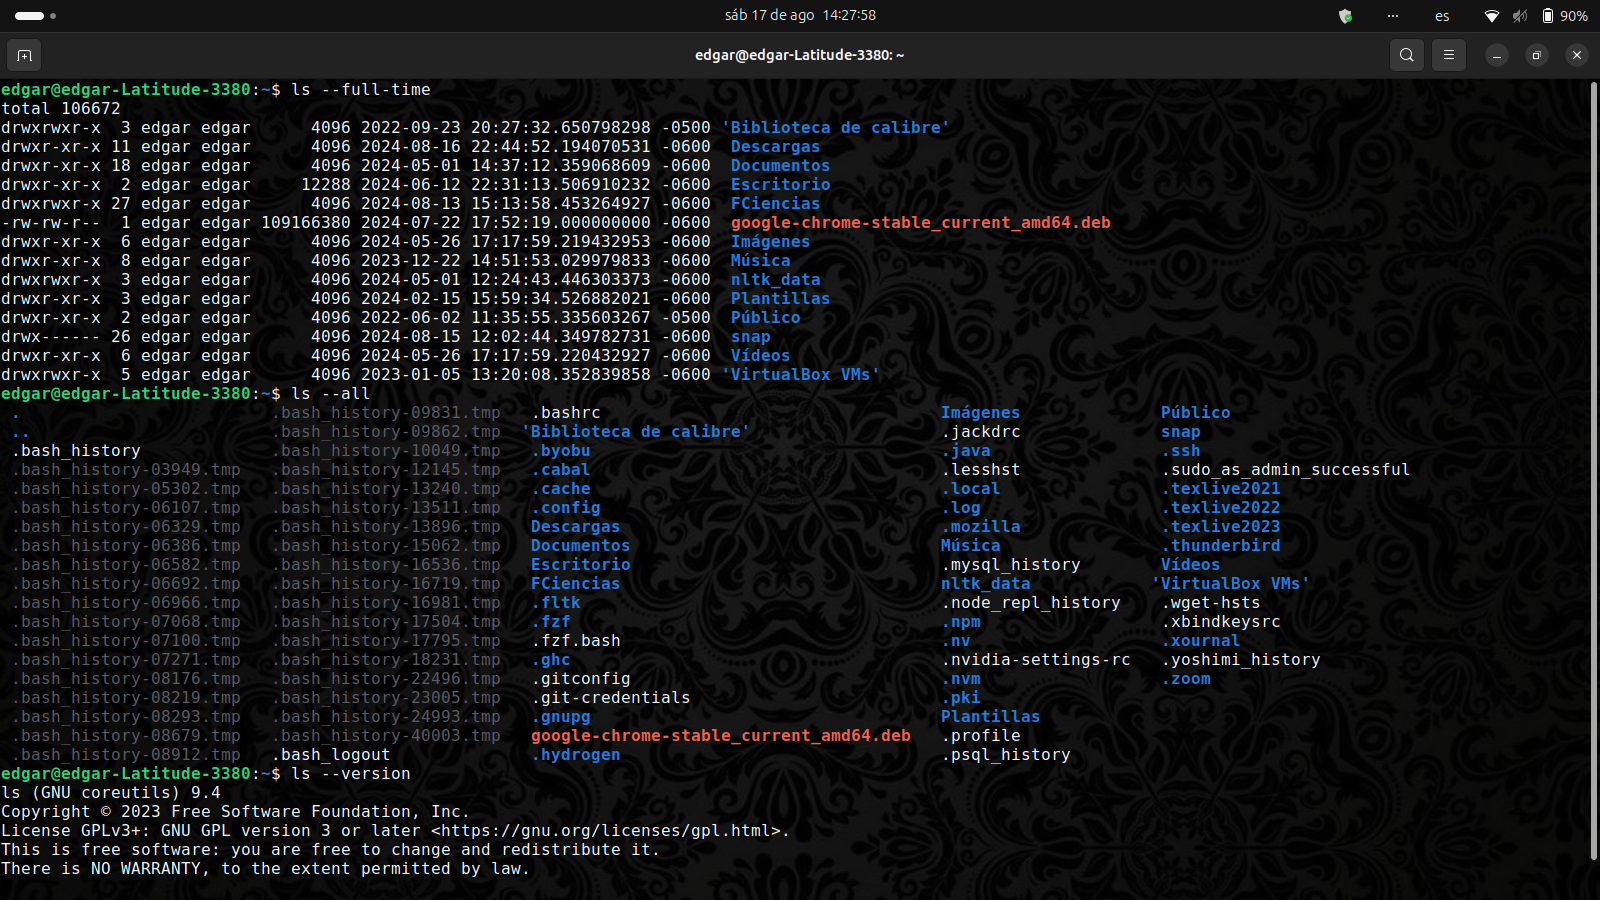
\includegraphics[width=10cm]{IMAGE/ls.png}
    \end{center}
    \begin{itemize}
        \item \texttt{ls --full-time}: Muestra detalles completos de archivos, incluyendo fecha y hora con segundos.
        \item \texttt{ls -al}: Lista todos los archivos, incluidos los ocultos, en un formato detallado.
        \item \texttt{ls --version}: Muestra la versión del comando \texttt{ls}.
    \end{itemize}

    
    \item \textbf{man} con al menos 3 banderas adicionales
    \begin{center}
        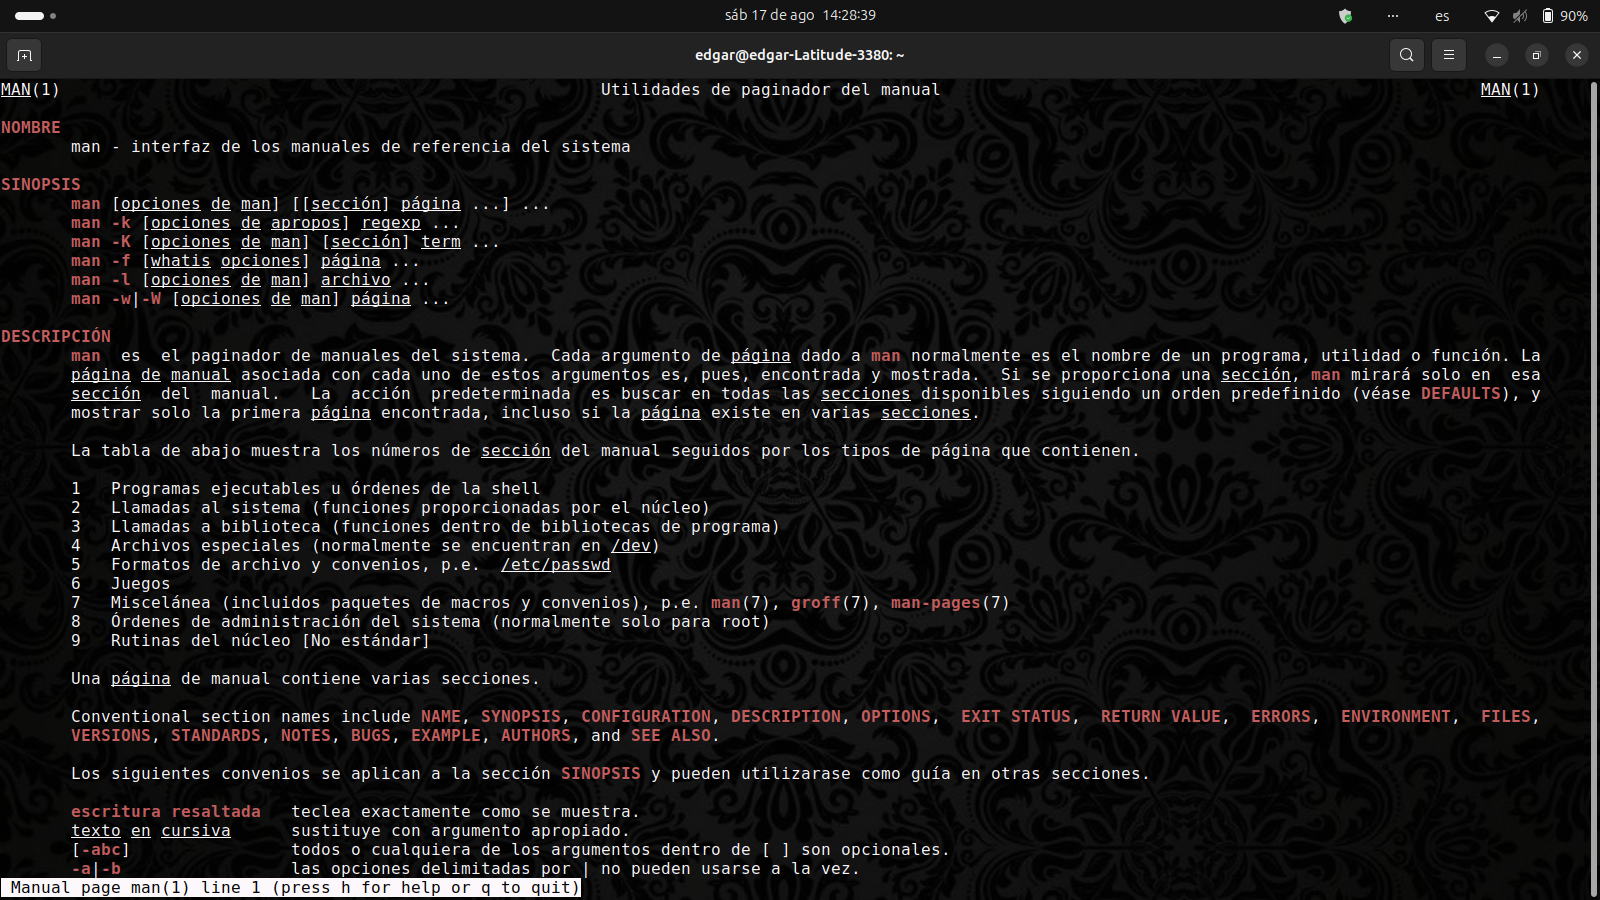
\includegraphics[width=10cm]{IMAGE/man-man.png}
    \end{center}
    \begin{center}
        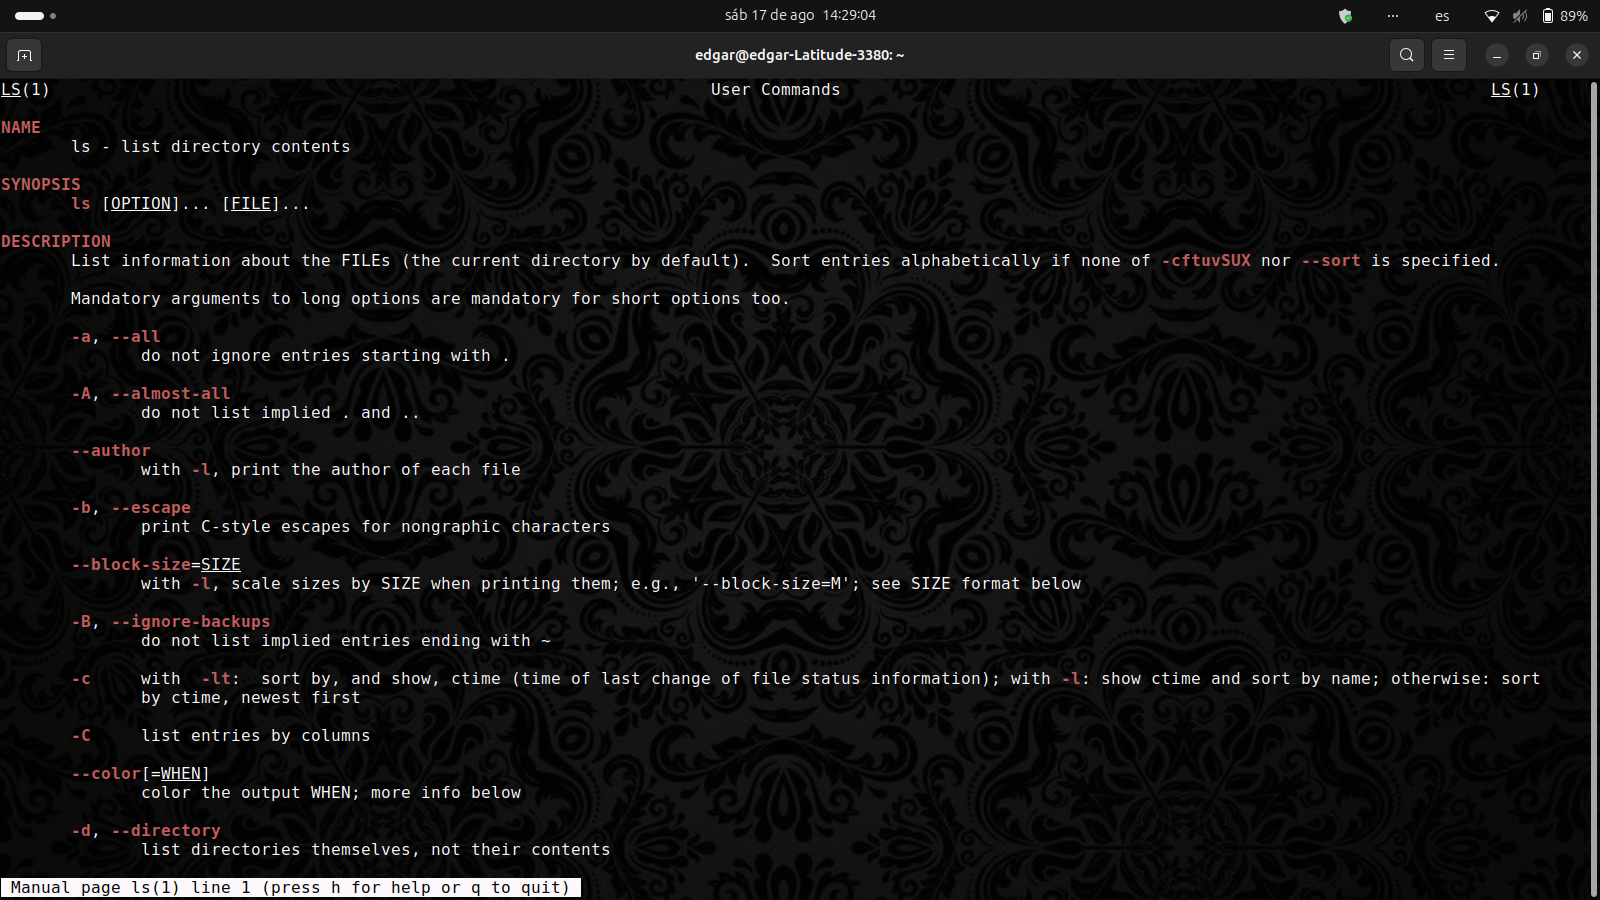
\includegraphics[width=10cm]{IMAGE/man-ls.png}
    \end{center}
    \begin{center}
        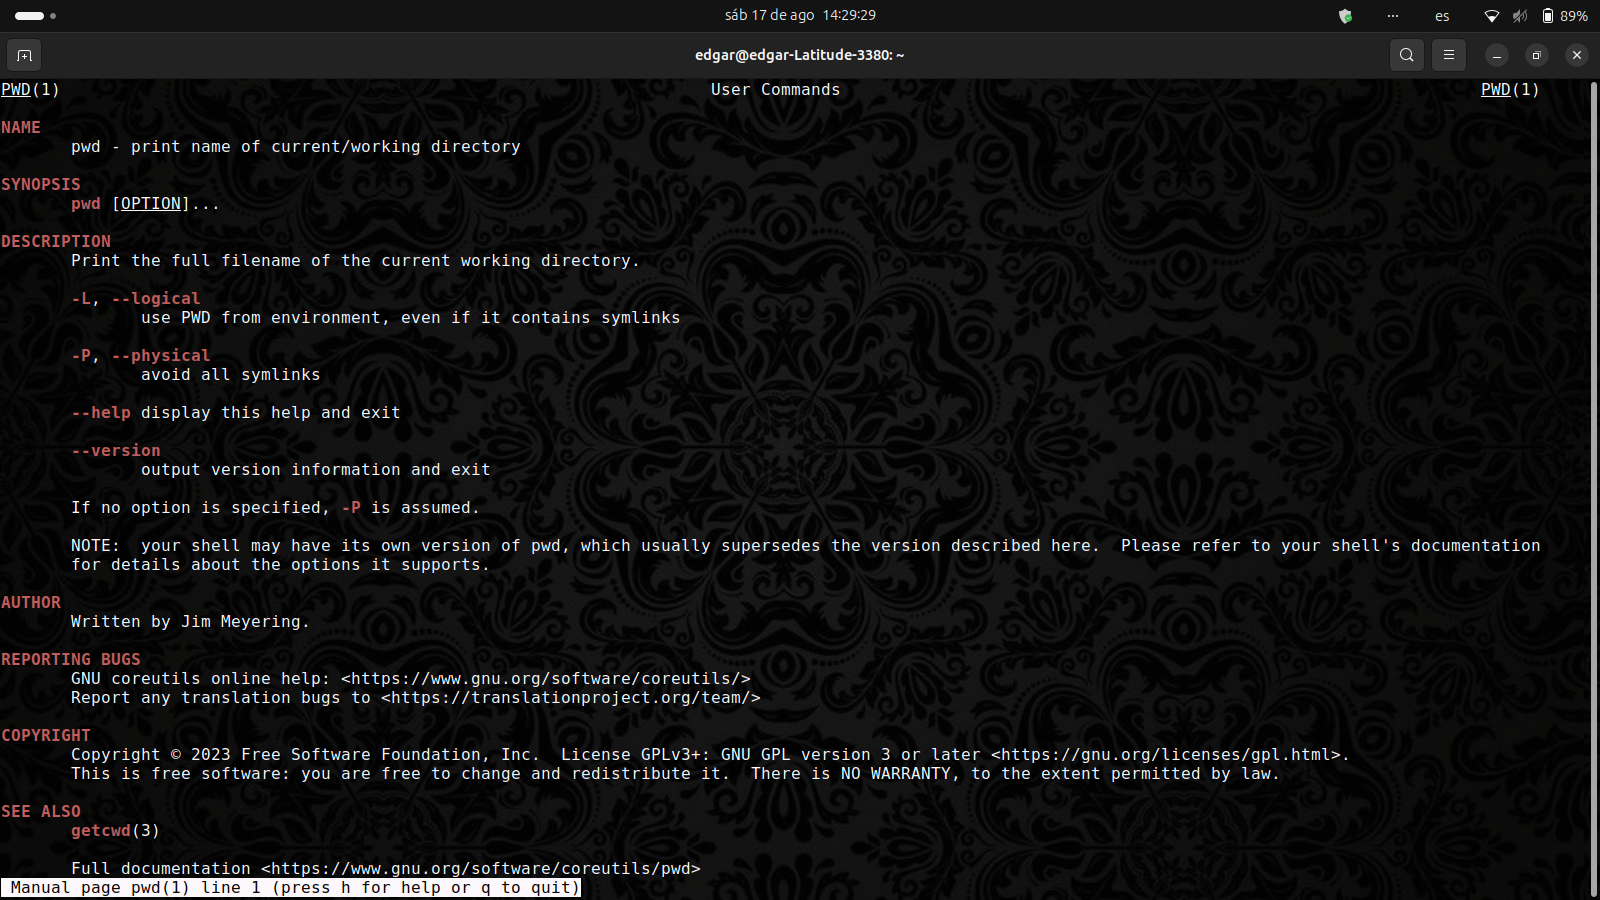
\includegraphics[width=10cm]{IMAGE/man-pwd.png}
    \end{center}
    \begin{itemize}
        \item \texttt{man man}: Muestra el manual del comando \texttt{man}, explicando cómo usar el sistema de páginas de manual.
        \item \texttt{man ls}: Muestra el manual del comando \texttt{ls}, detallando sus opciones y uso.
        \item \texttt{man pwd}: Muestra el manual del comando \texttt{pwd}, que describe cómo obtener el directorio de trabajo actual.
    \end{itemize}

    \item \textbf{mkdir} con 3 banderas \\
    El comando mkdir se utiliza para crear directorios. Y las banderas modifican su comportamiento.\\
    \begin{itemize}
        \item mkdir -v: Muestra un mensaje por cada directorio creado.\\	
        \item mkdir -p: Crea directorios padres si no existen.\\
        \item mkdir -m: Permite asignar permisos al directorio creado.\\
        \item mkdir --help: Muestra la ayuda del comando.\\
    \end{itemize}
    \begin{center}
            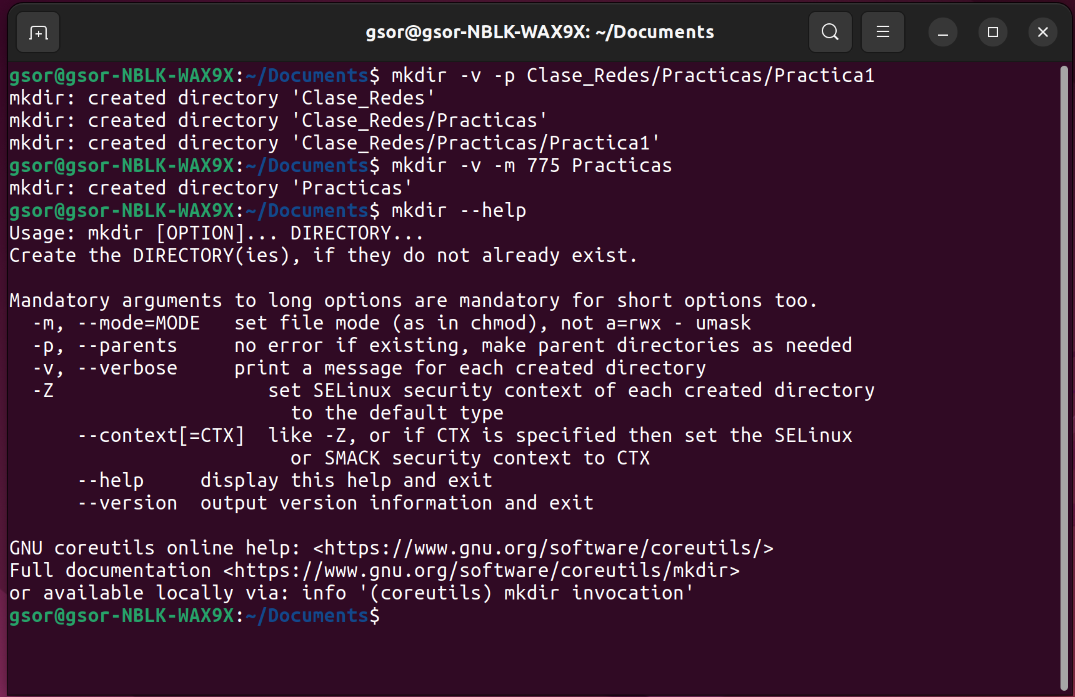
\includegraphics[width=10cm]{IMAGE/comandos/mkdir_examples.png}\\
    \end{center}
    \item \textbf{cp} con al menos 3 banderas
    El comando cp se utiliza para copiar archivos o directorios.\\
    \begin{itemize}
        \item cp -v: Muestra un mensaje por cada archivo copiado.\\
        \item cp -s: Crea un enlace simbólico en lugar de copiar el archivo.\\
        \item cp -t <directorio>: Copia los archivos al directorio especificado.\\
        \item cp -r <directorio>: Copia un directorio y su contenido.\\
    \end{itemize}
    \begin{center}
        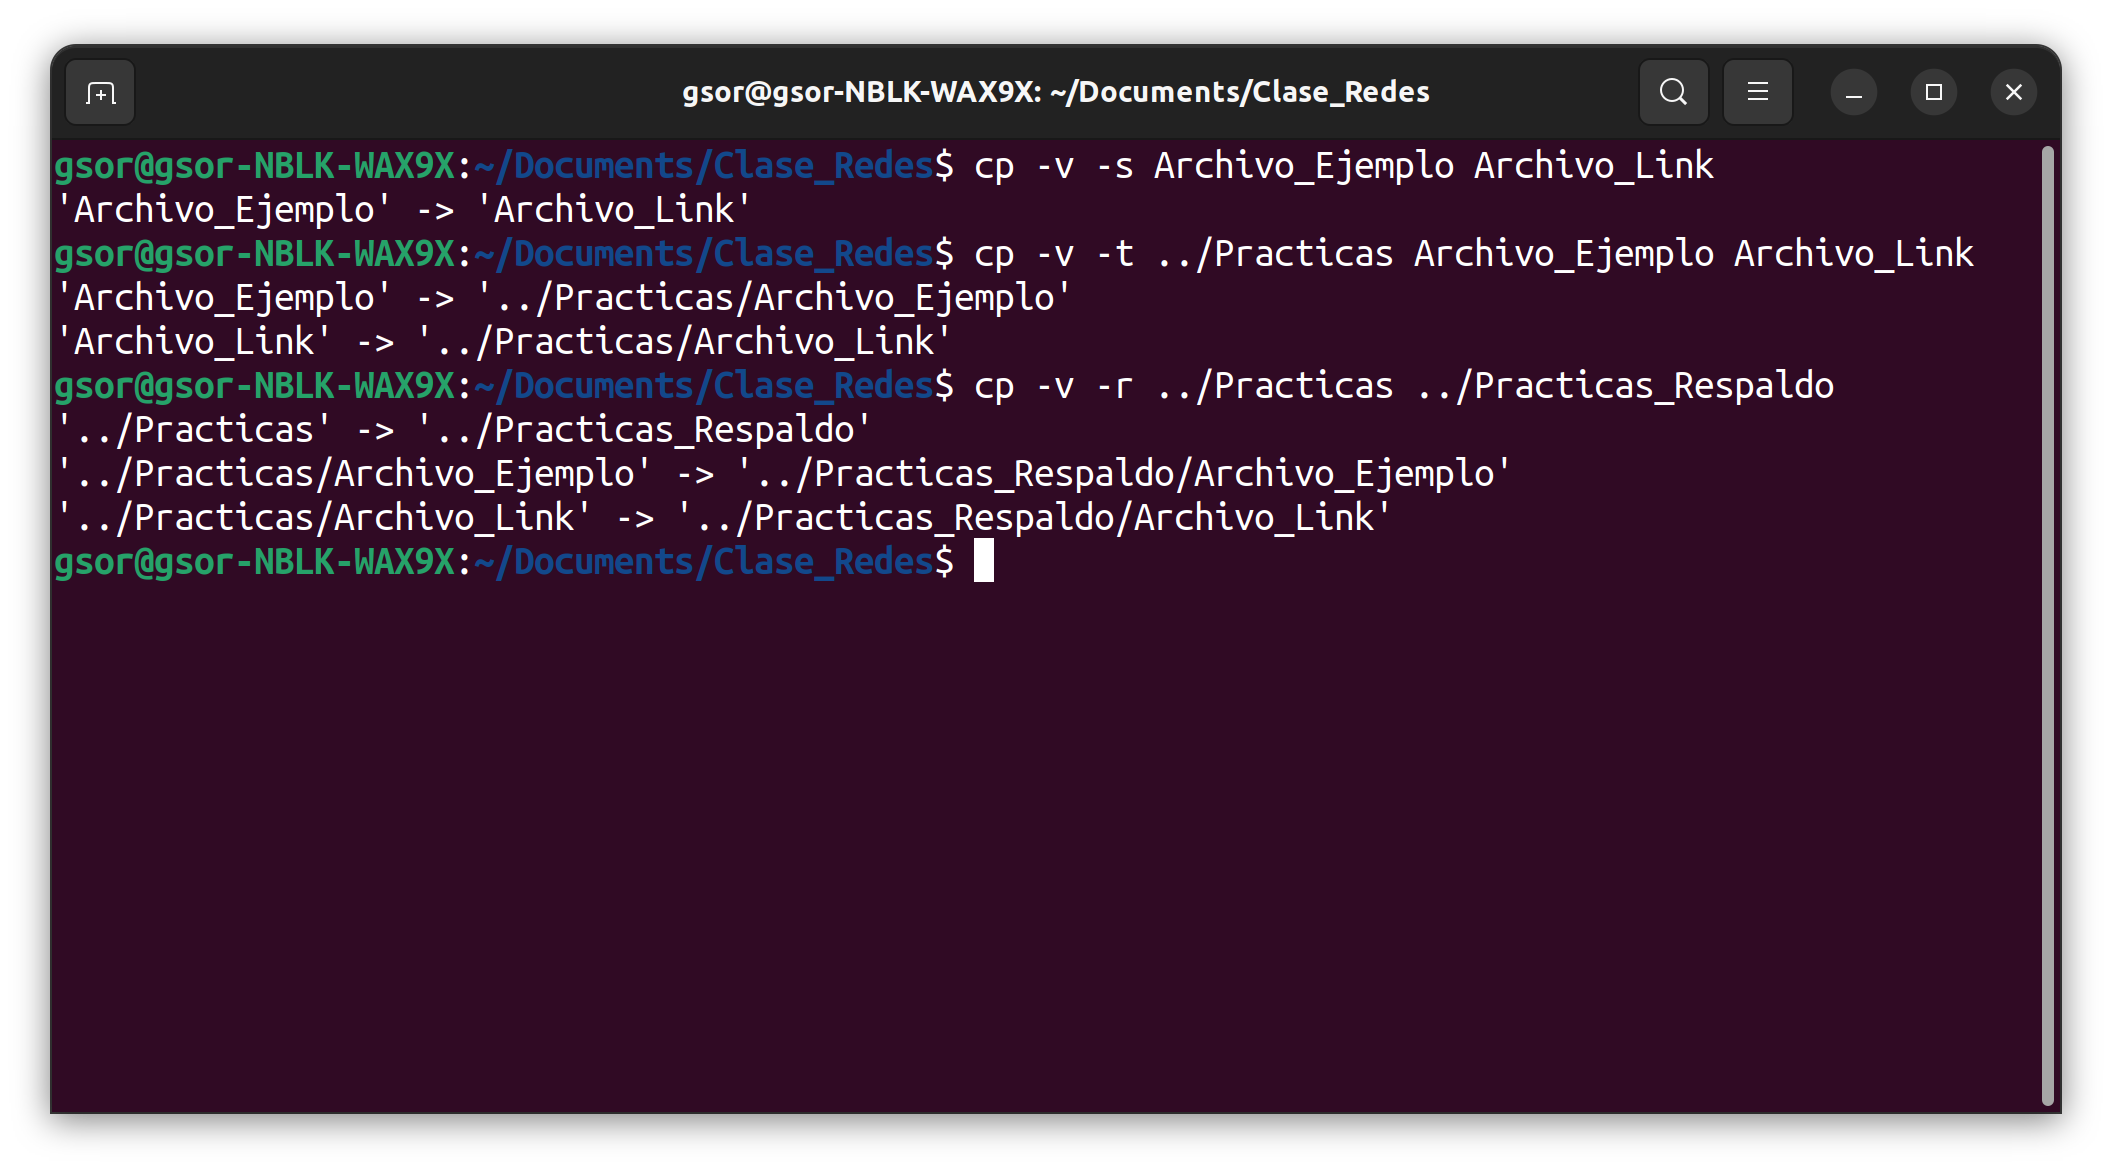
\includegraphics[width=10cm]{IMAGE/comandos/cp_examples.png}\\
    \end{center}
    \item \textbf{mv} con al menos 3 banderas. \\
	Su función principal es mover archivos de un directorio a otro.  También puede renombrar archivos o carpetas. \\
	-v: Explica lo que hace el comando y lo ejecuta.\\
	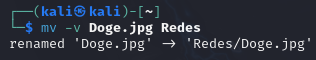
\includegraphics[]{IMAGE/Ejercicio1/mv1.png}\\
	-t: Mueve diferentes archivos a un directorio, primero se escribe el directorio y después los archivos.\\
	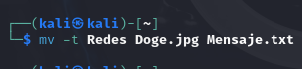
\includegraphics[]{IMAGE/Ejercicio1/mv2.png}\\
	-i: En caso de que el archivo a mover/renombrar ya exista en el directorio destino, pregunta si se quiere sobreescribir.\\
	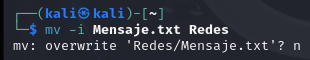
\includegraphics[]{IMAGE/Ejercicio1/mv3.png}\\
    \item \textbf{grep} con al menos 3 banderas. \\
	Su función es buscar un patrón que definamos en un archivo de texto, es decir buscar una o varias palabras en un 
	archivo y se imprimirá la línea o líneas que coincidan.\\
	-i: No distingue minúsculas de mayúsculas.\\
	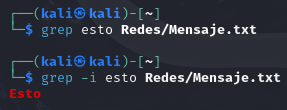
\includegraphics[]{IMAGE/Ejercicio1/grep1.png}\\
	-n: Indica el número de línea donde se encontró el patron.\\
	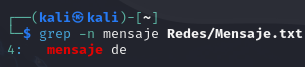
\includegraphics[]{IMAGE/Ejercicio1/grep2.png}\\
	-x: Encuentra el patron donde coincida la linea completa.\\
	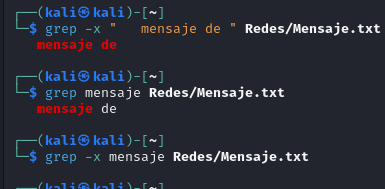
\includegraphics[]{IMAGE/Ejercicio1/grep3.png}\\
    \item \textbf{cat}\\
	Deriva de la palabra concatenar y permite crear, fusionar o imprimir archivos en la terminal.\\
	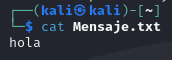
\includegraphics[]{IMAGE/Ejercicio1/cat.png}\\
    \item \textbf{head} (con alguna configuración)\\
	Sirve para mostrar el inicio de un archivo de texto.\\
	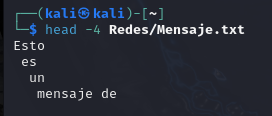
\includegraphics[]{IMAGE/Ejercicio1/head.png}\\
    \item \textbf{less} (con alguna configuración)
    Es un visor de archivos que permite desplazarse por el contenido de un archivo de texto.\\
    \begin{itemize}
        \item less -N:  Muestra los números de línea junto al contenido del archivo.\\
    \end{itemize}
    \begin{center}
        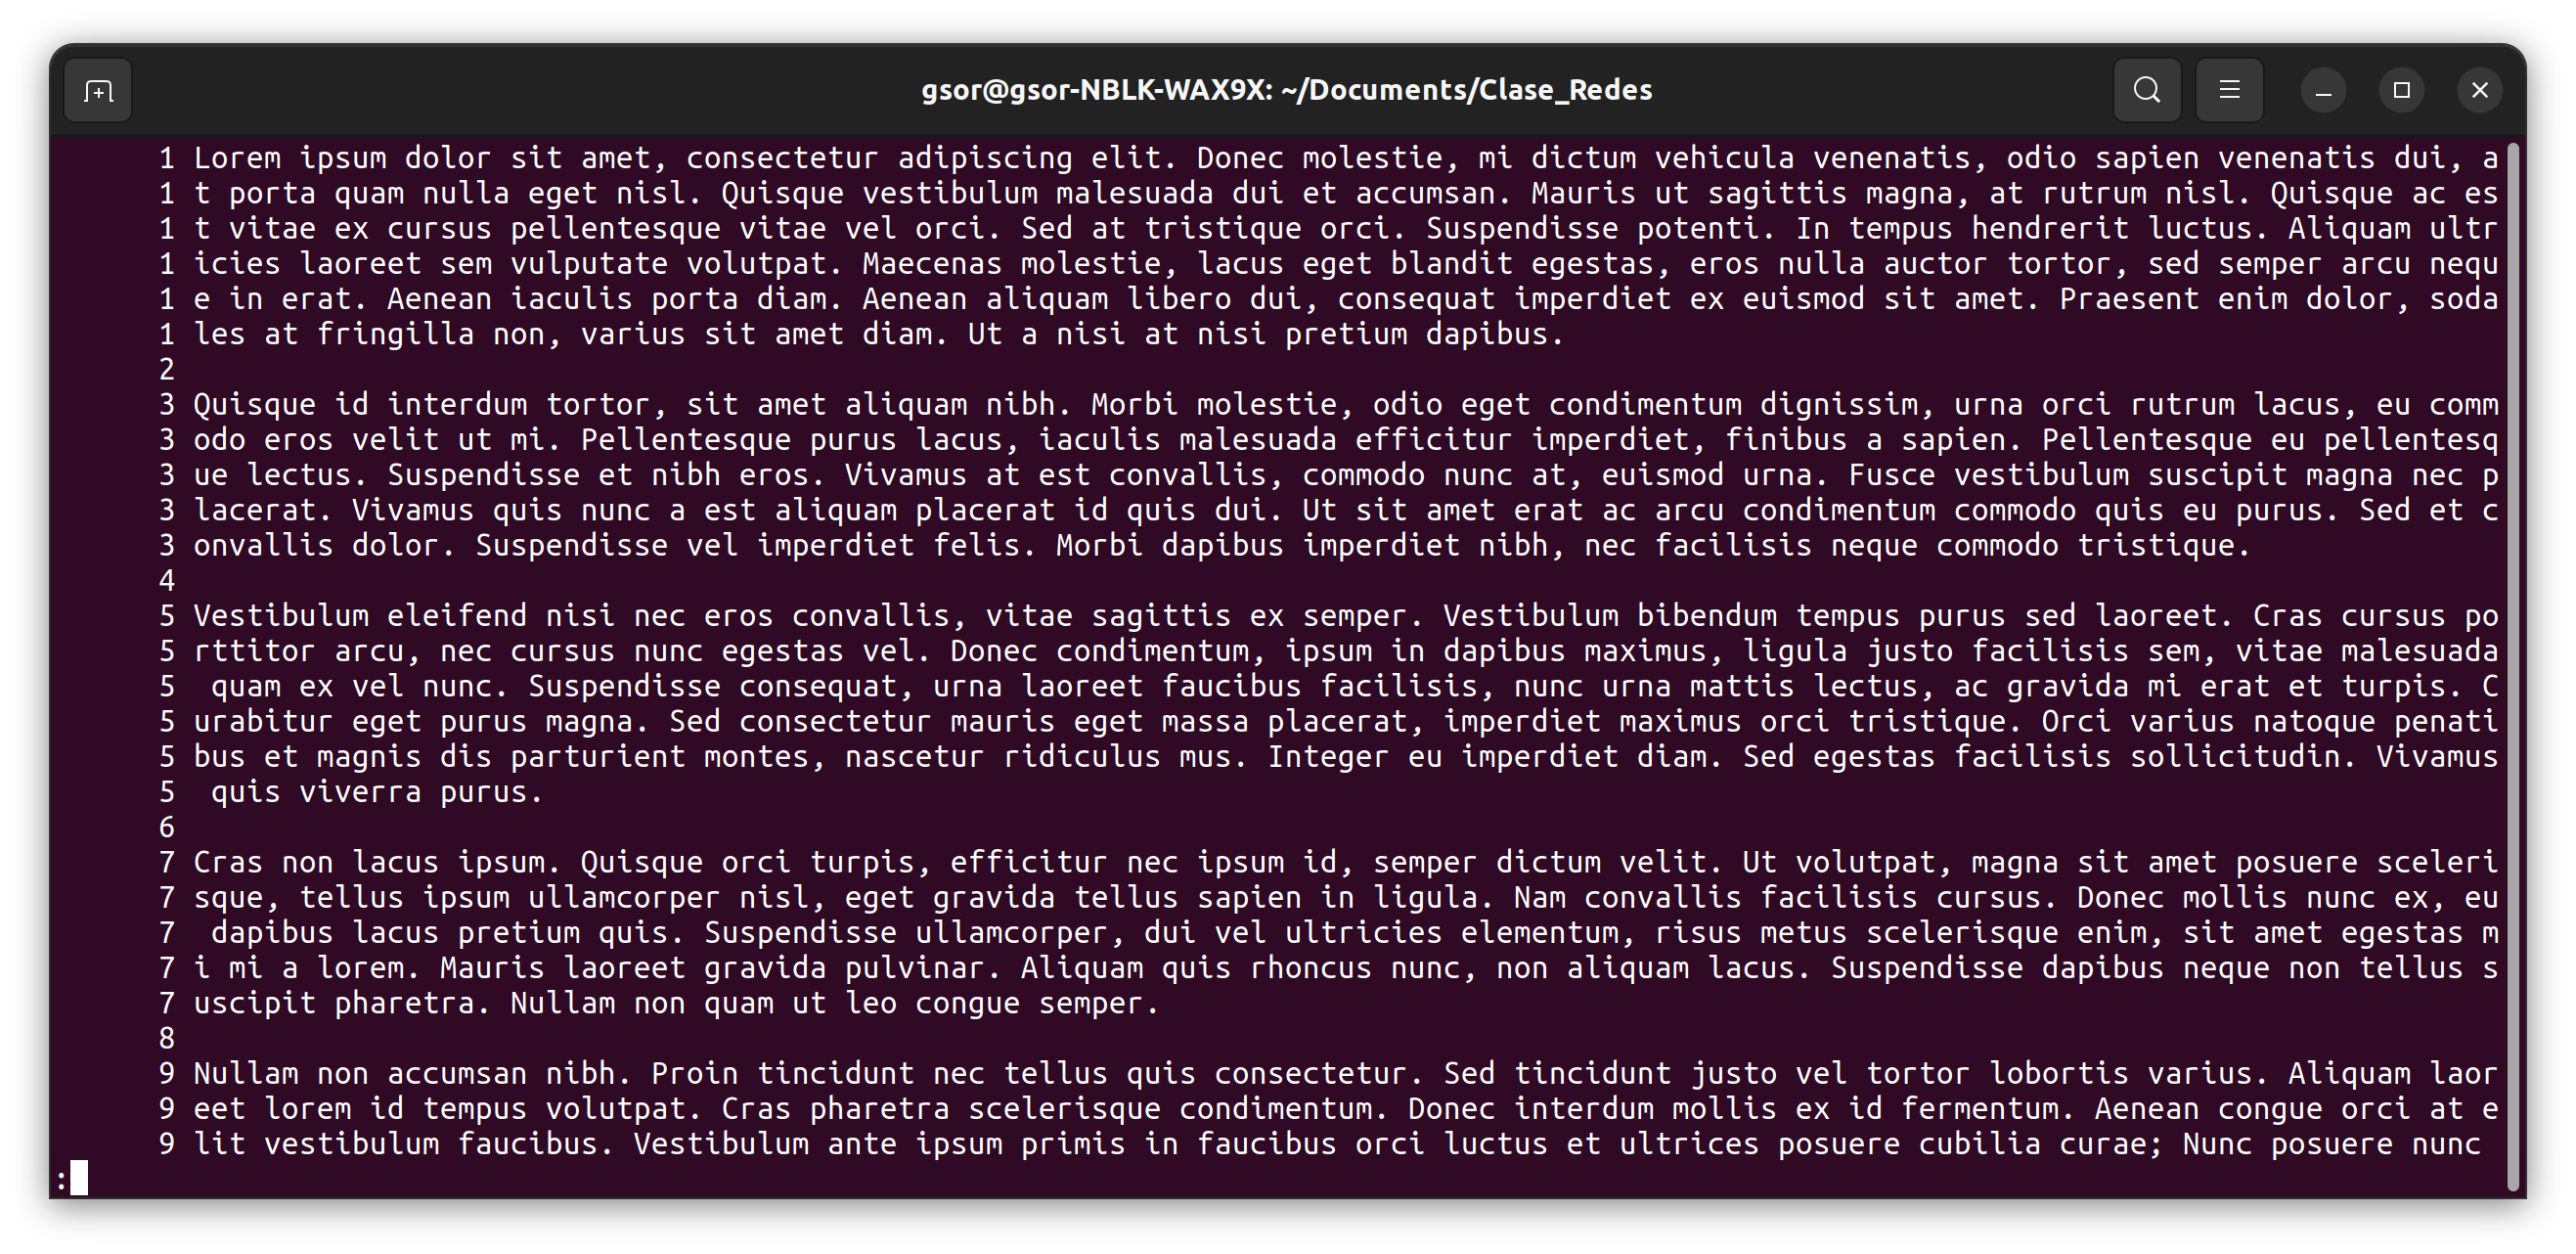
\includegraphics[width=10cm]{IMAGE/comandos/less-example.png}\\
    \end{center}
    \item \textbf{find}\\
    Busca archivos que cumplan las condiciones que especifique el usuario, comenzando por el directorio que nombre. Por ejemplo, si quiere buscar nombres de archivos que concuerden con determinado patrón o que hayan sido modificados durante un periodo de tiempo determinado.\\
    \begin{center}
        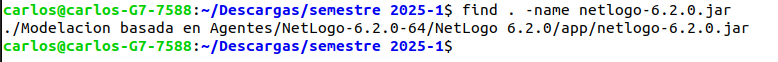
\includegraphics[width=12cm]{IMAGE/find.png}
    \end{center}
    
    \item \textbf{uniq}\\
    Permite obtener líneas únicas de un archivo o entrada dada. Elimina líneas consecutivas duplicadas, dejando solo una de ellas.
    \begin{center}
        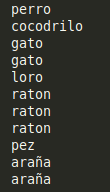
\includegraphics[width=2cm]{IMAGE/lista.png}
    \end{center}
    
    \begin{center}
        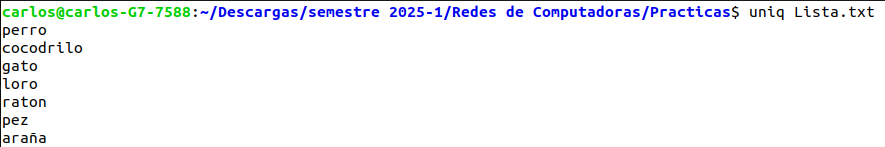
\includegraphics[width=13cm]{IMAGE/uniq.png}
    \end{center}
    
    \item \textbf{ps}; ¿Qué significará PID y TTY?\\
    Muestra una lista con todos los procesos que se estén ejecutando en el sistema en ese momento, con su identificador del proceso (PID), terminal asociado (TTY), tiempo de uso de CPU (TIME) y nombre del ejecutable (CMD).
    \begin{center}
        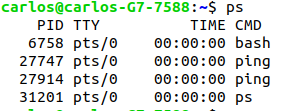
\includegraphics[width=5cm]{IMAGE/ps.png}
    \end{center}
    \item \textbf{kill}, ¿Tendrá relación con \textbf{ps}?
    El comando kill se utiliza para enviar una señal a un proceso, por lo general para detenerlo.\\
    \begin{itemize}
        \item less -N:  Muestra los números de línea junto al contenido del archivo.\\
    \end{itemize}
    \begin{center}
         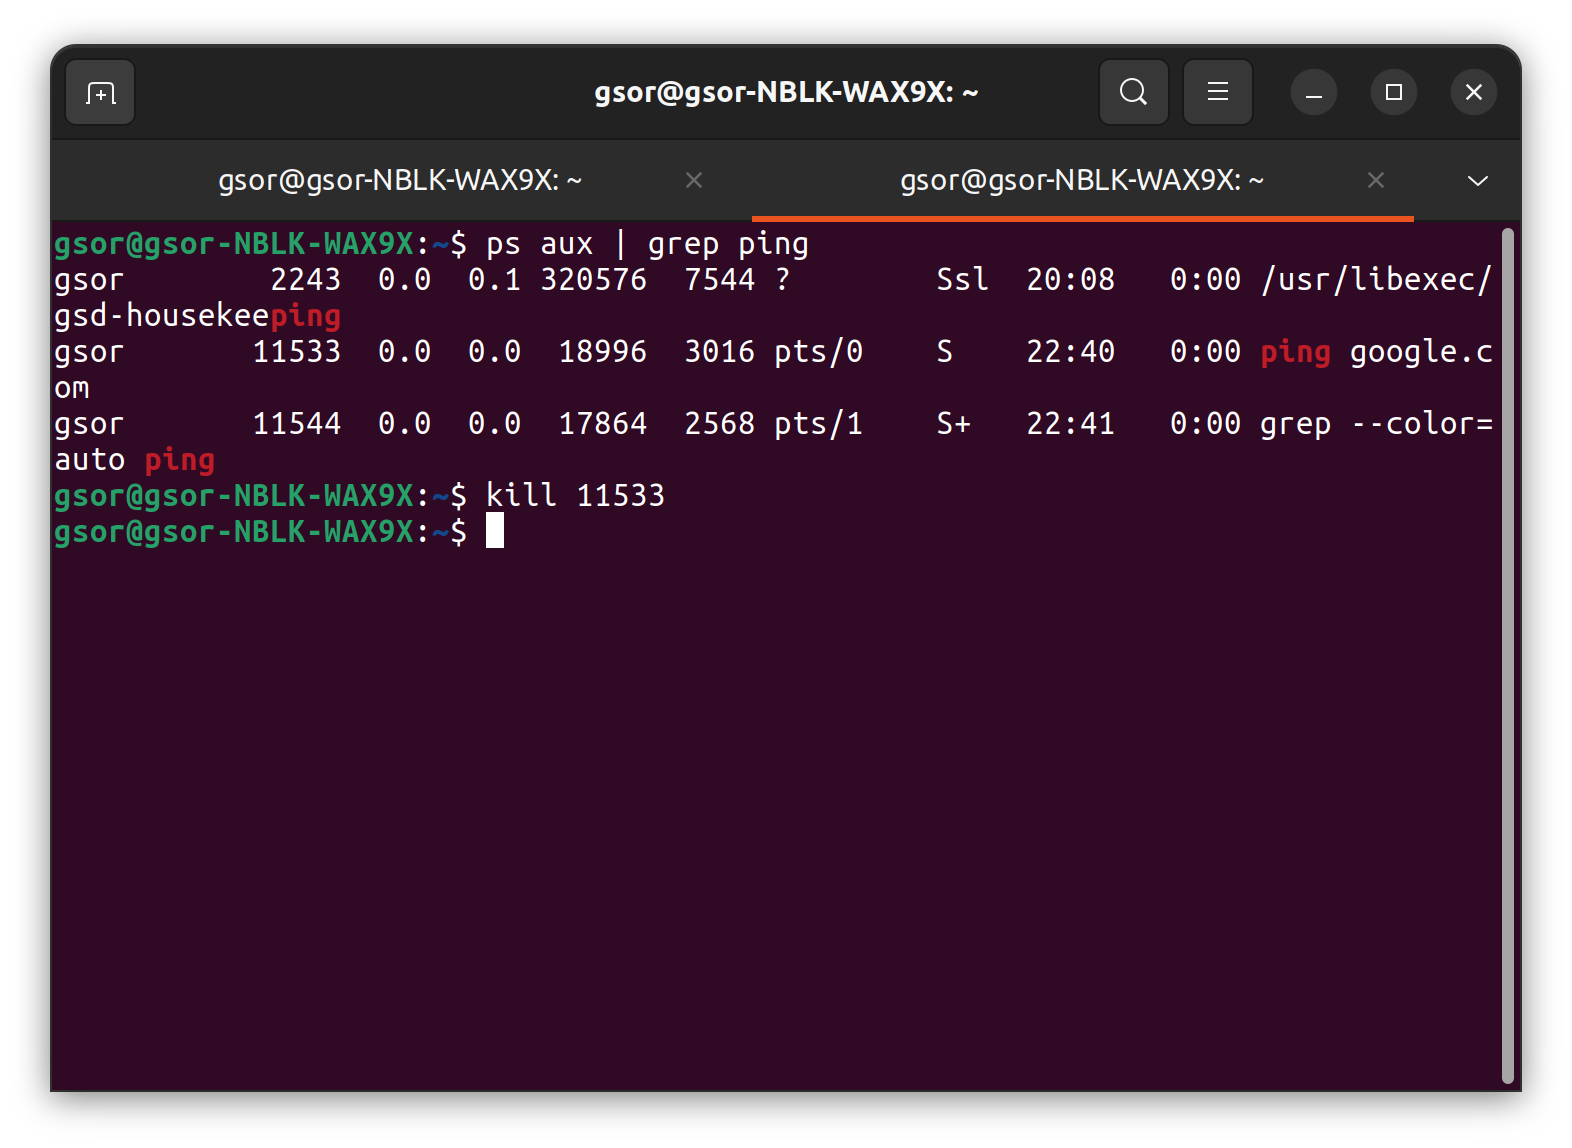
\includegraphics[width=10cm]{IMAGE/comandos/kill.png}\\
    \end{center}
    Para poder usar el comando kill es necesario conocer el PID del proceso que se desea detener, para ello se usa el comando ps.\\
    \item \textbf{1}
    El comando df se utiliza para mostrar el espacio disponible en los sistemas de archivos.\\
    \begin{itemize}
        \item df -h: Muestra el espacio disponible en los sistemas de archivos en un formato legible para el usuario.\\
        \item df -T: Muestra el tipo de sistema de archivos.\\
        \item df -i: Muestra el número de inodos disponibles. Un inodo es una estructura de datos utilizada por los sistemas de archivos 
        en Unix y Linux para almacenar información sobre un archivo o un directorio. \\
    \end{itemize}
    \begin{center}
        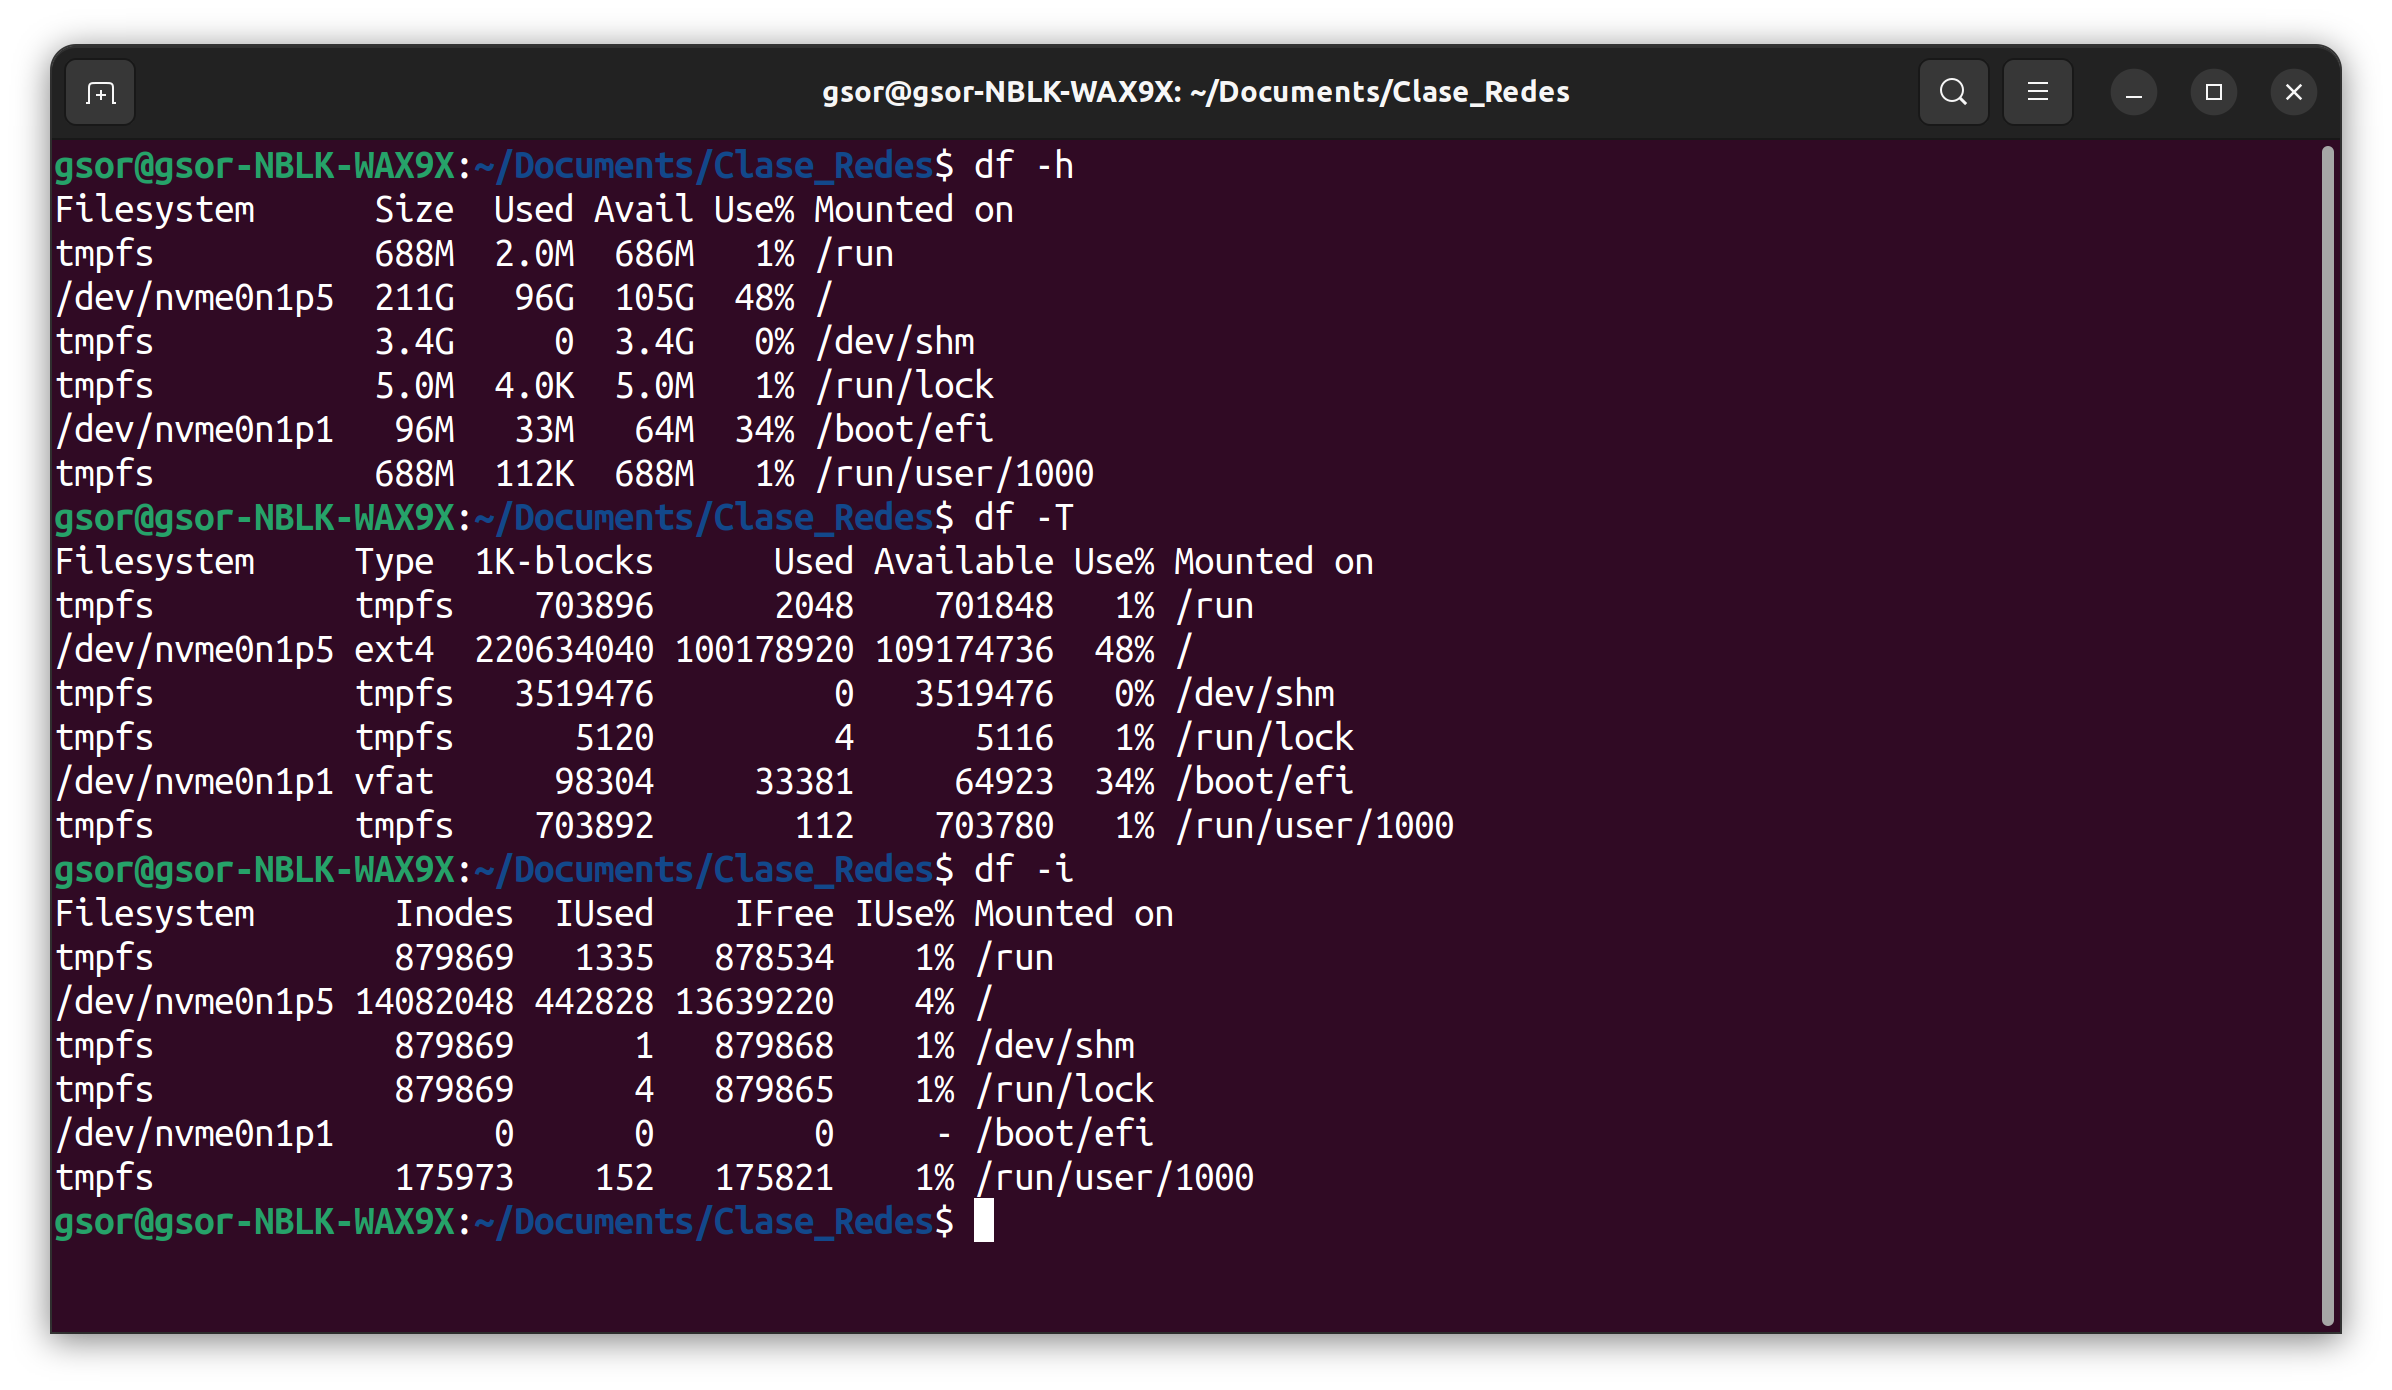
\includegraphics[width=10cm]{IMAGE/comandos/df.png}\\
    \end{center}
    \item \textbf{2}
    El comando curl se utiliza para transferir datos desde o hacia un servidor.\\
    \begin{itemize}
        \item curl -I: Muestra solo la cabecera de la respuesta del servidor.\\
        \item curl -o: Guarda la salida en un archivo en un archivo de texto.\\
        \item curl -L: Sigue redirecciones.\\ 
    \end{itemize}
    \begin{center}
        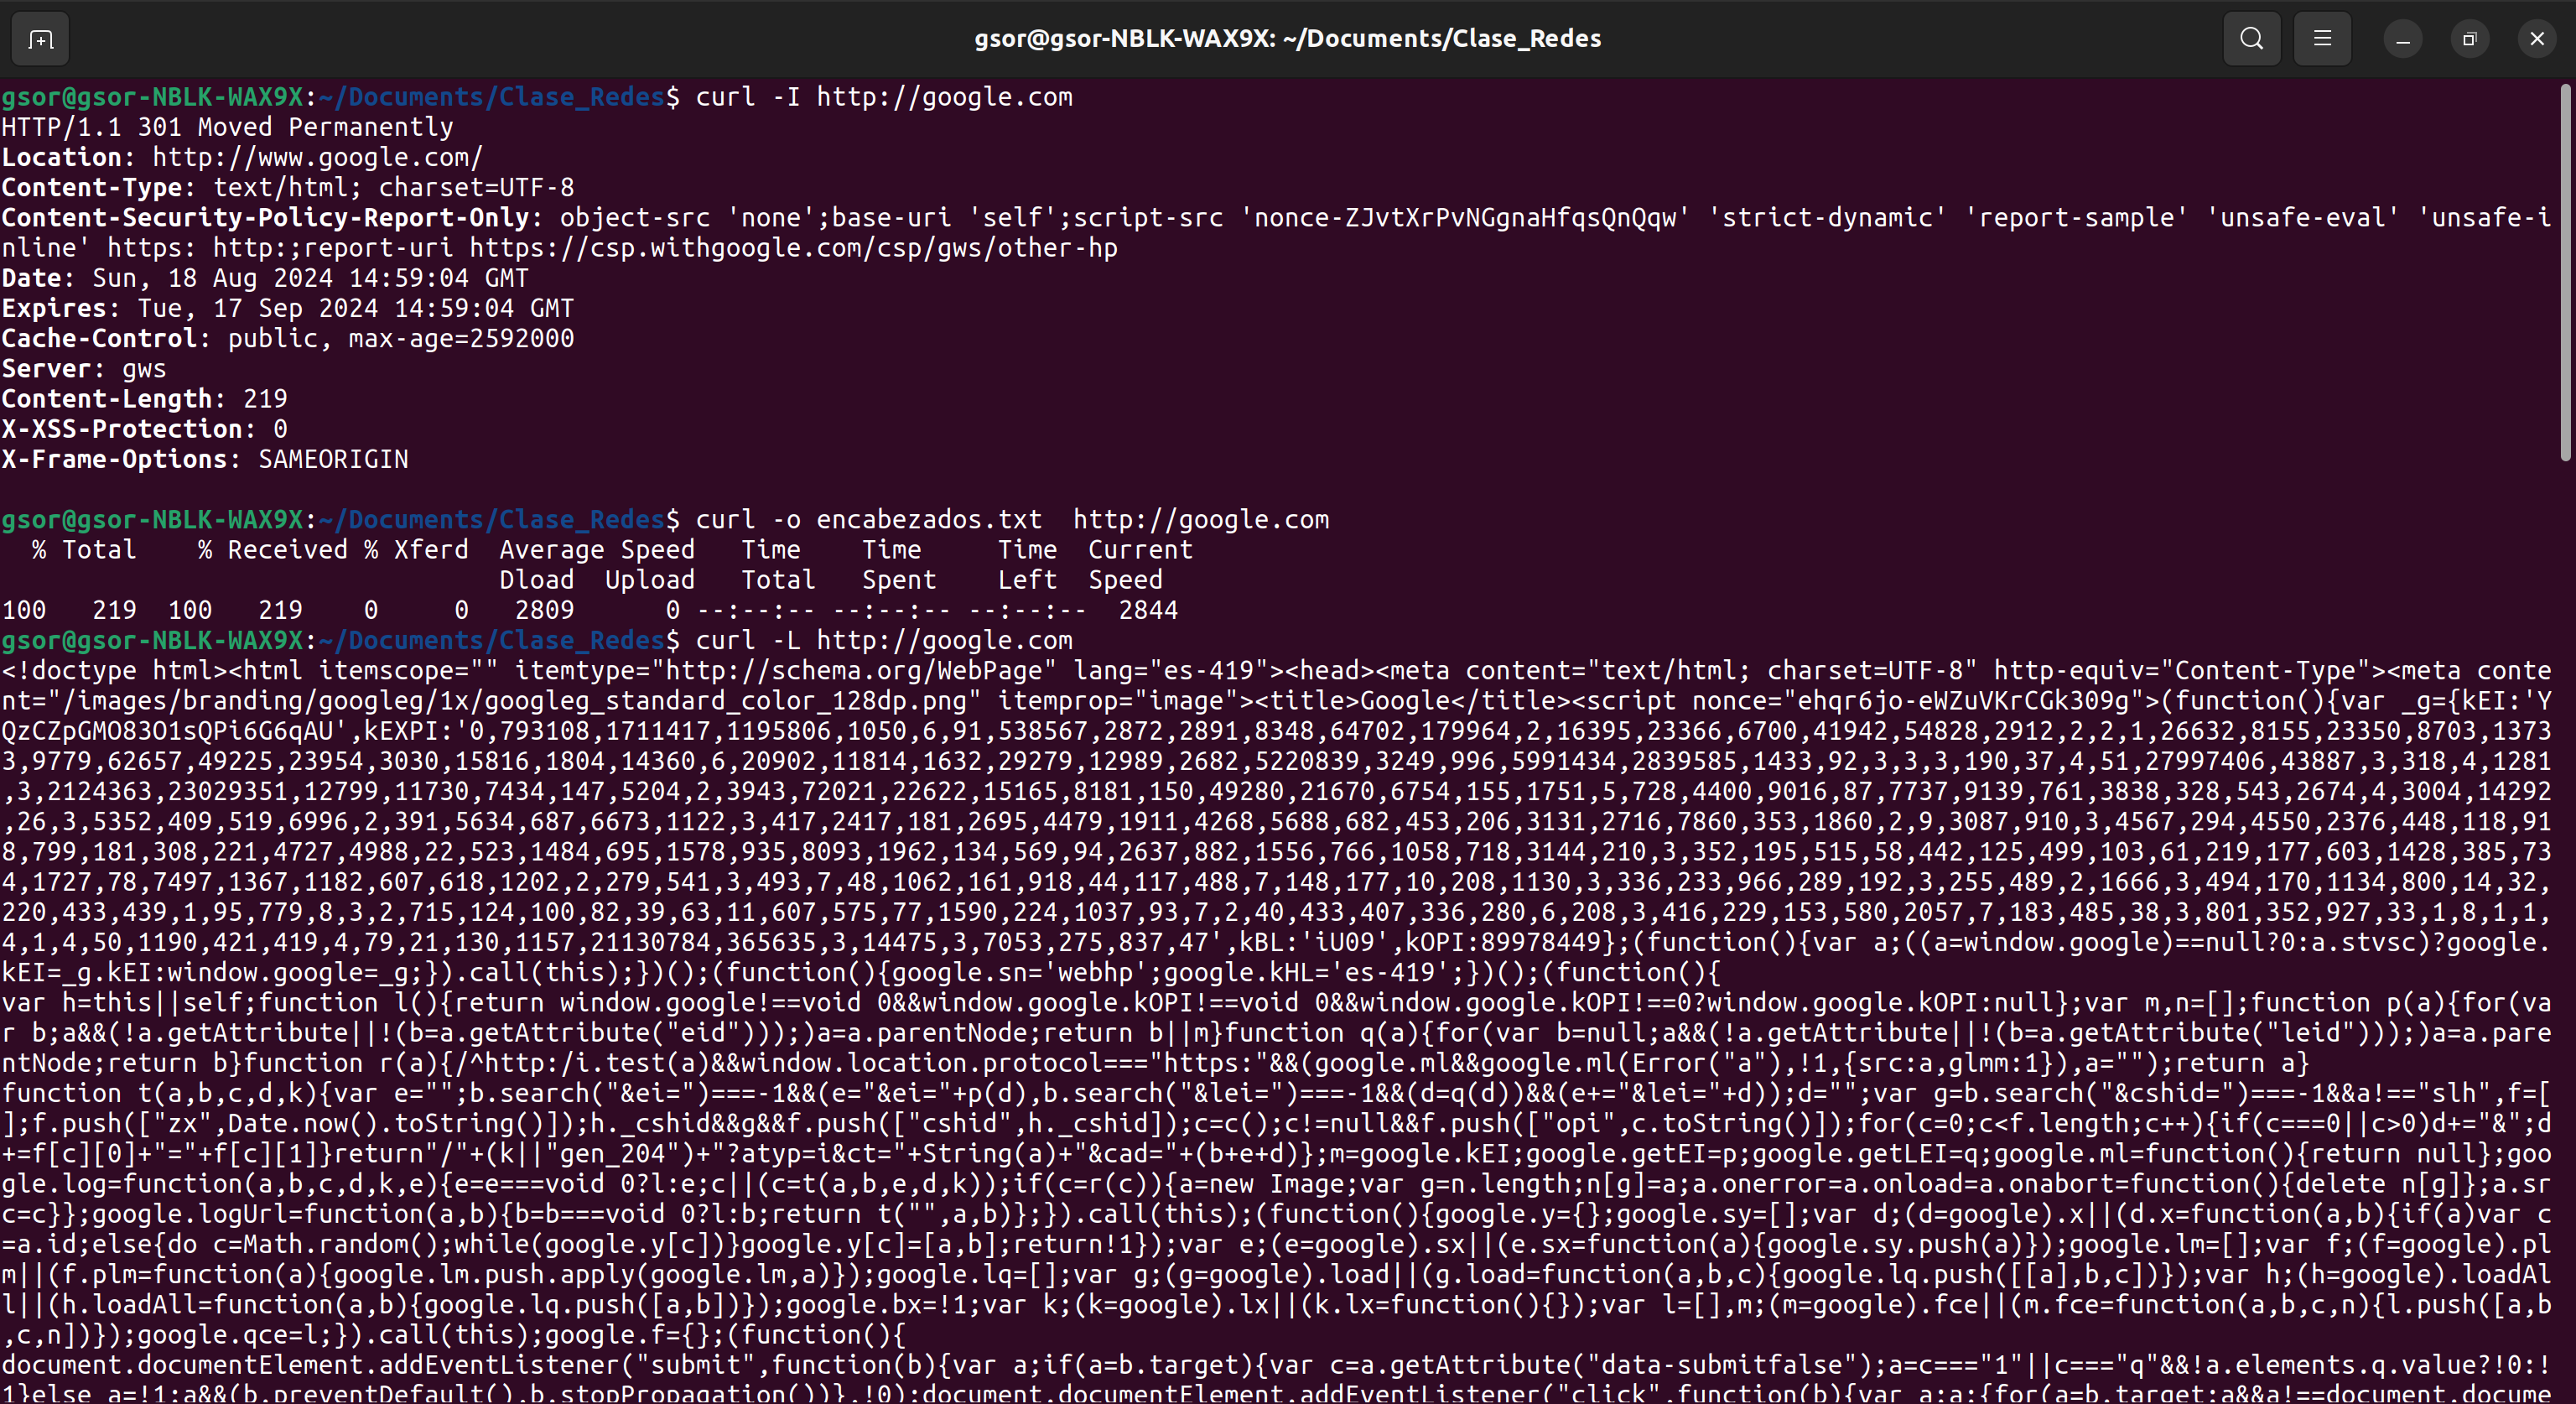
\includegraphics[width=10cm]{IMAGE/comandos/curl.png}\\
    \end{center}
    \item \textbf{3}
    El comando sort se utiliza para ordenar líneas de texto en un archivo.\\
    \begin{itemize}
        \item sort -r: Ordena las líneas en orden inverso.\\
        \item sort -n: Ordena las líneas numéricamente.\\
        \item sort -k <número>: Ordena las líneas por la columna especificada.\\         
    \end{itemize}
    \begin{center}
        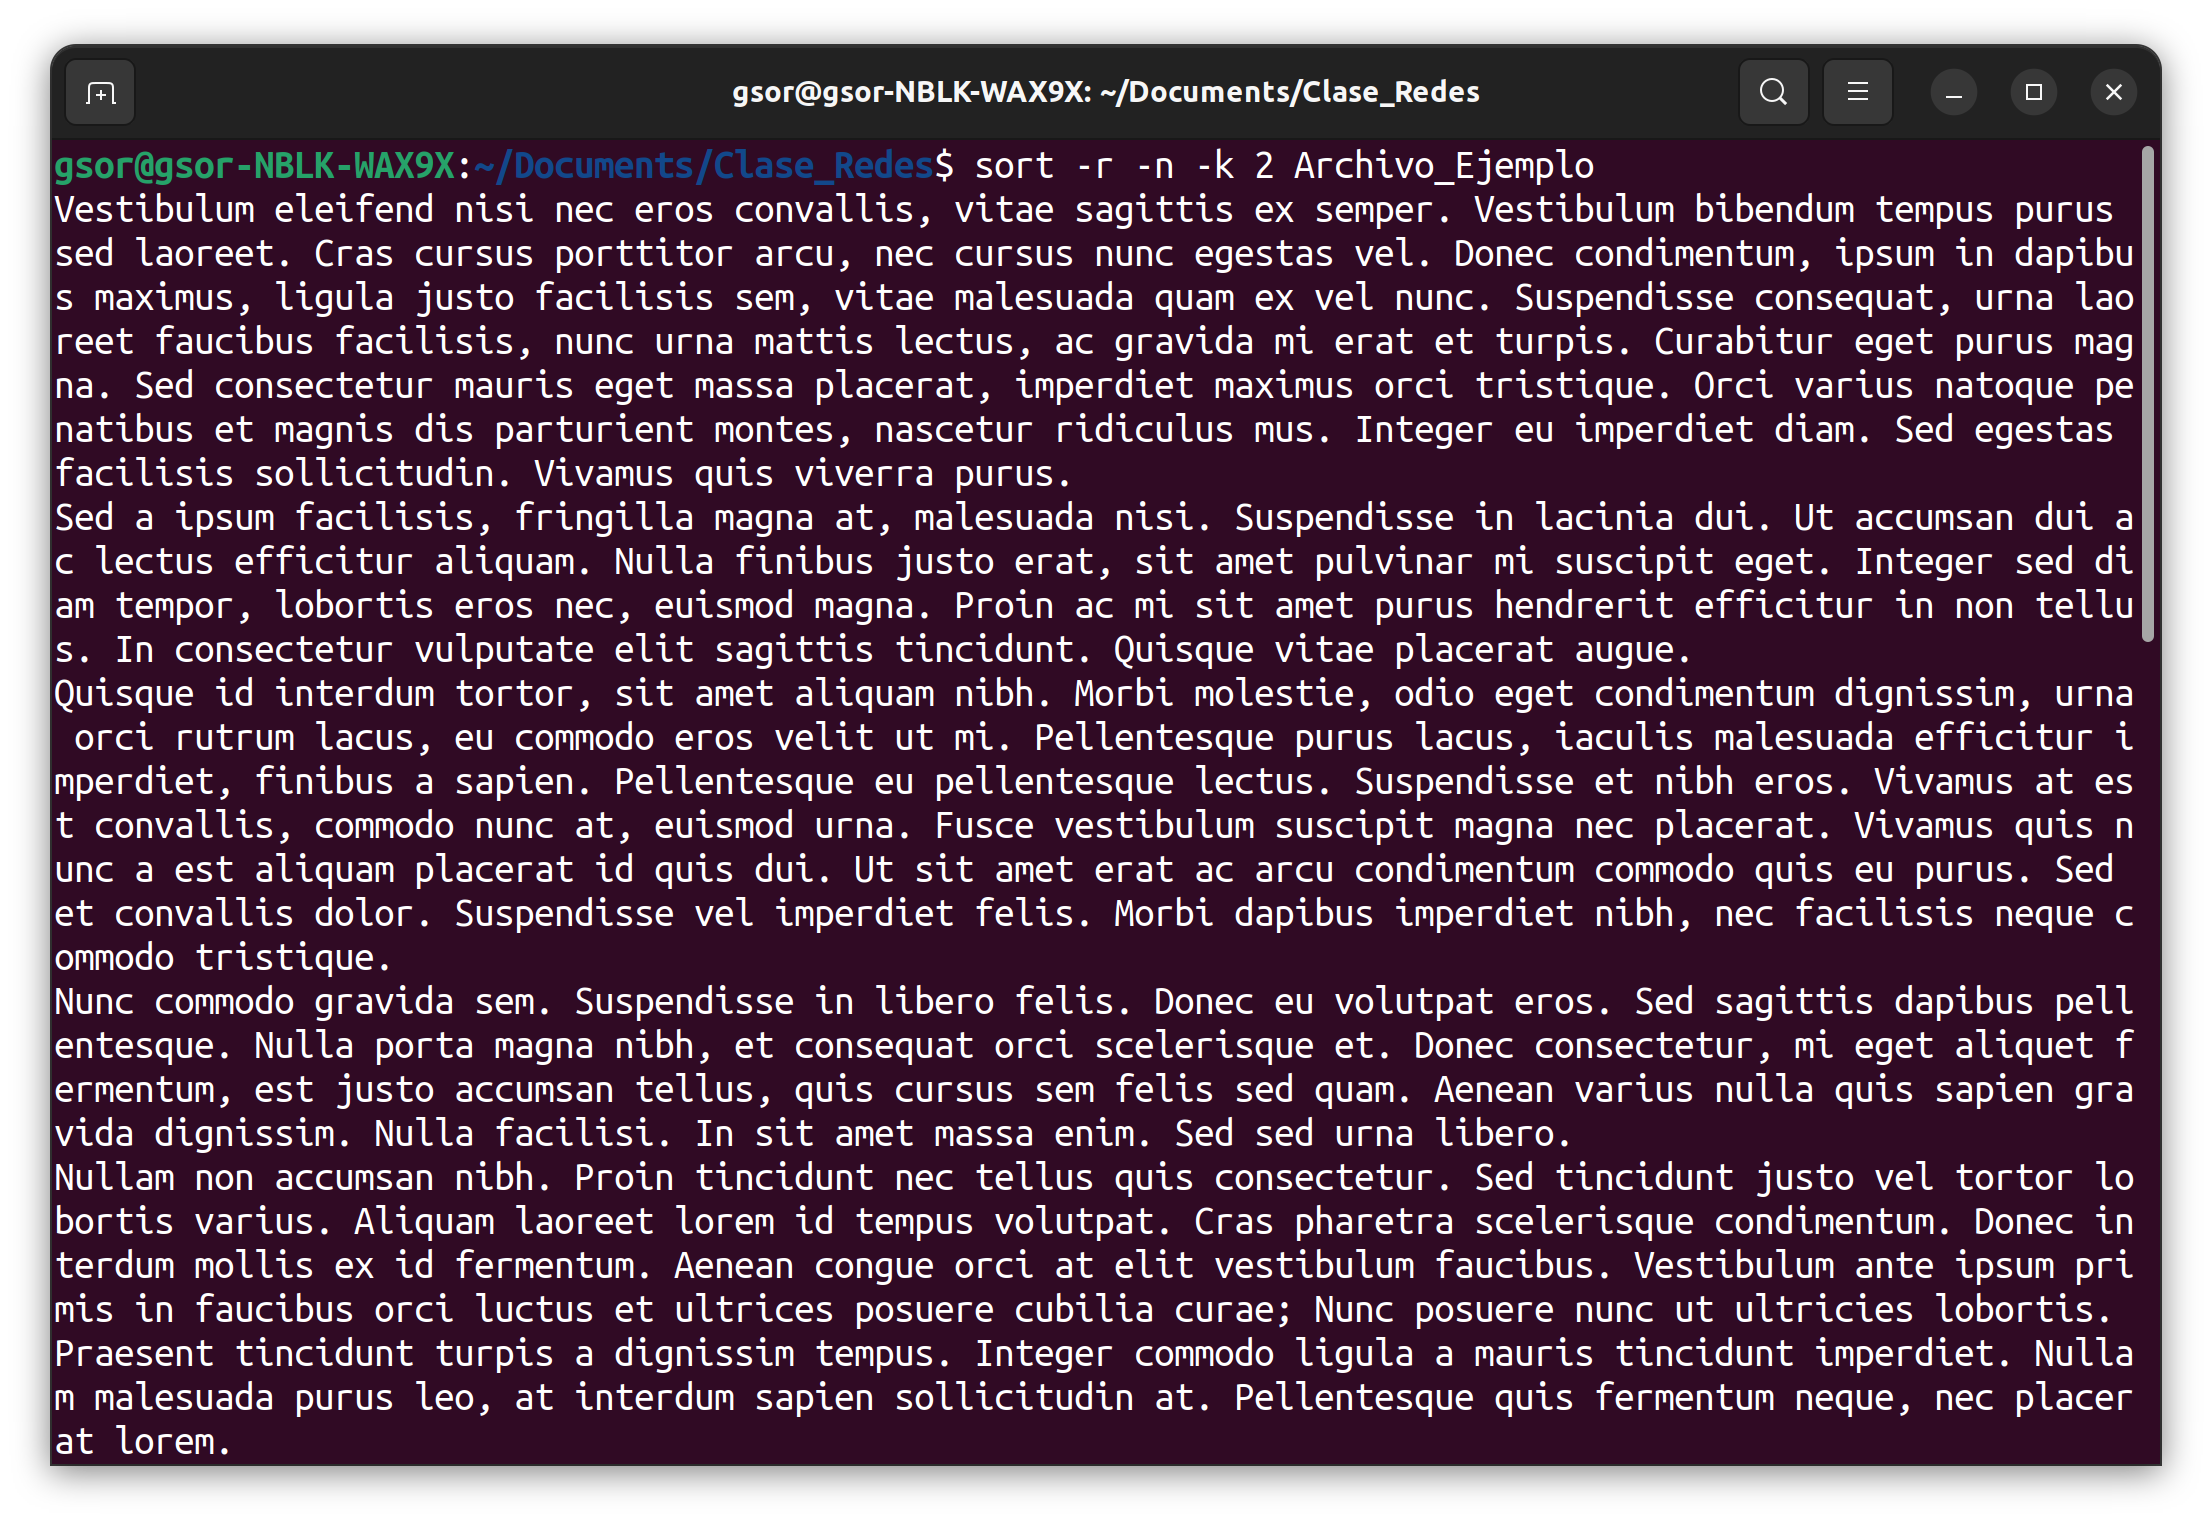
\includegraphics[width=10cm]{IMAGE/comandos/sort.png}\\
    \end{center}
    \item \textbf{4}
    El comando tar se utiliza para comprimir y descomprimir archivos.\\
    \begin{itemize}
        \item tar -c: Crea un archivo comprimido.\\
        \item tar -v : Muestra los archivos que se están comprimiendo o descomprimiendo.\\
        \item tar -f <archivo>: Especifica el nombre del archivo comprimido.\\
        \item tar -z: Comprime o descomprime el archivo con gzip.\\
        \item tar -x: Descomprime un archivo.\\
    \end{itemize}
    \begin{center}
        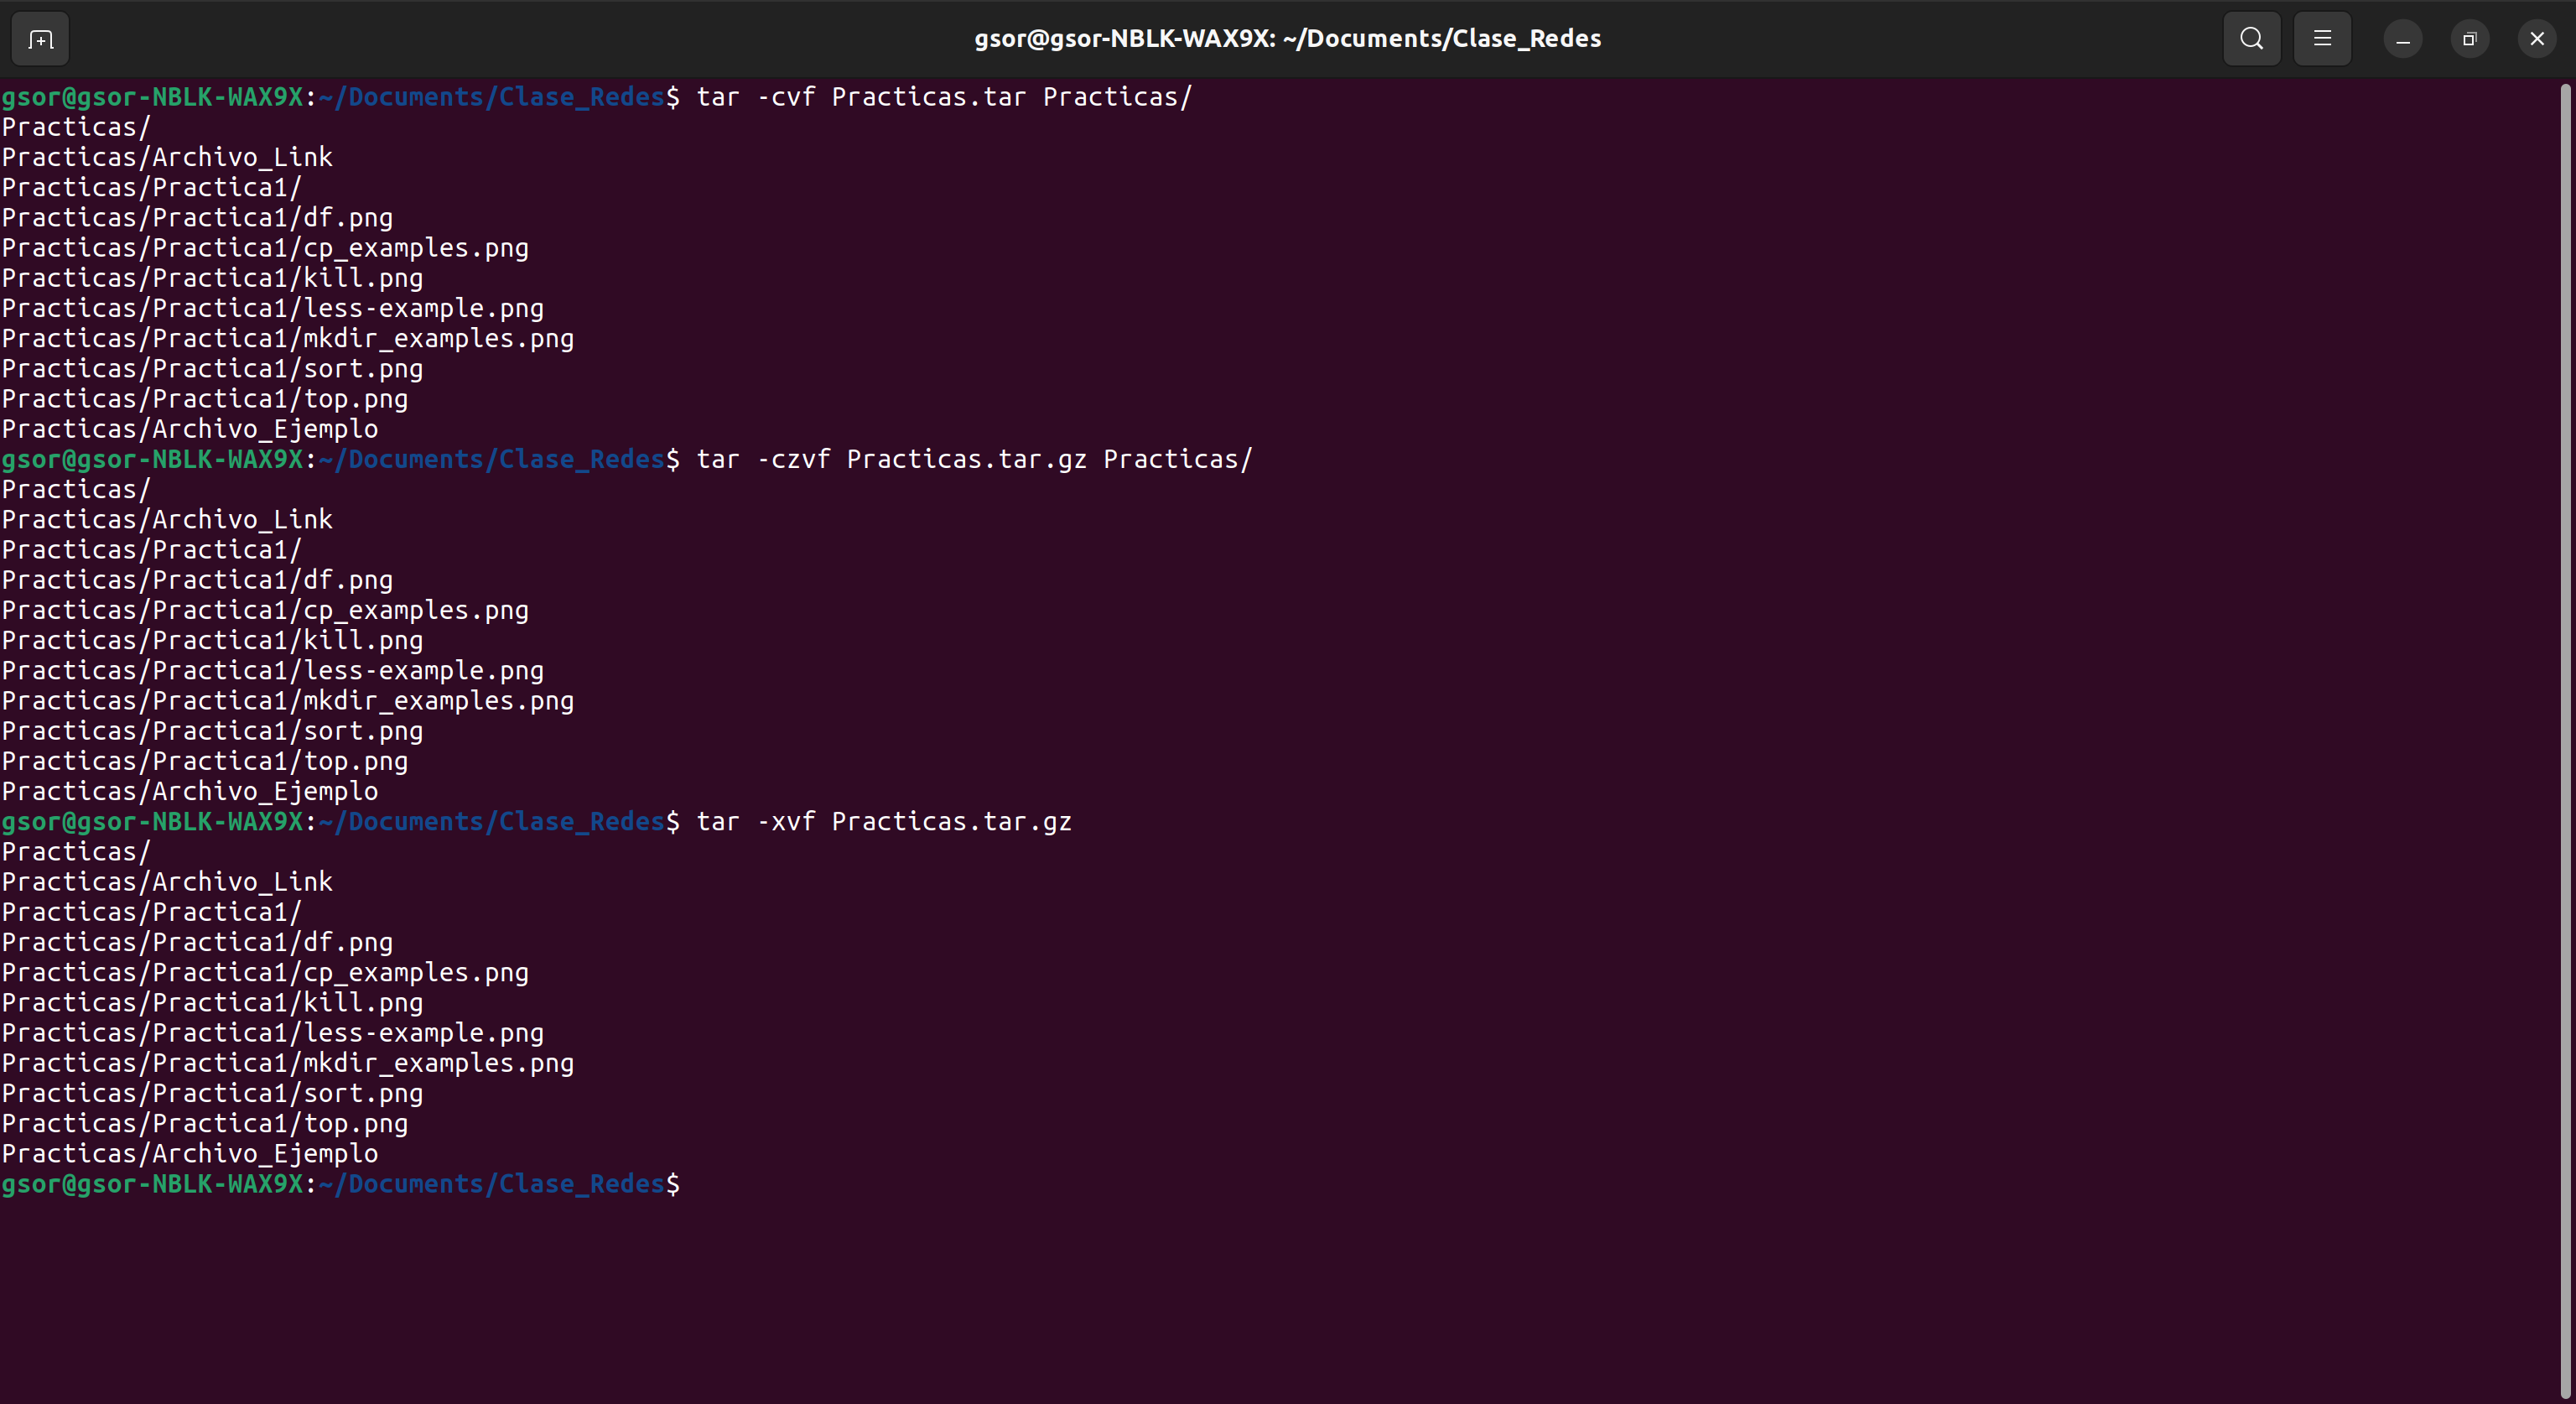
\includegraphics[width=10cm]{IMAGE/comandos/tar.png}\\
    \end{center}
    \item \textbf{5}
    El comando top se utiliza para mostrar los procesos en ejecución en el sistema.\\
    \begin{itemize}
        \item top -d <número>: Actualiza la información cada n segundos.\\
        \item top -u <usuario>: Muestra los procesos del usuario especificado.\\
        \item top -b : Muestra la información en modo batch.\\
    \end{itemize}
    \begin{center}
        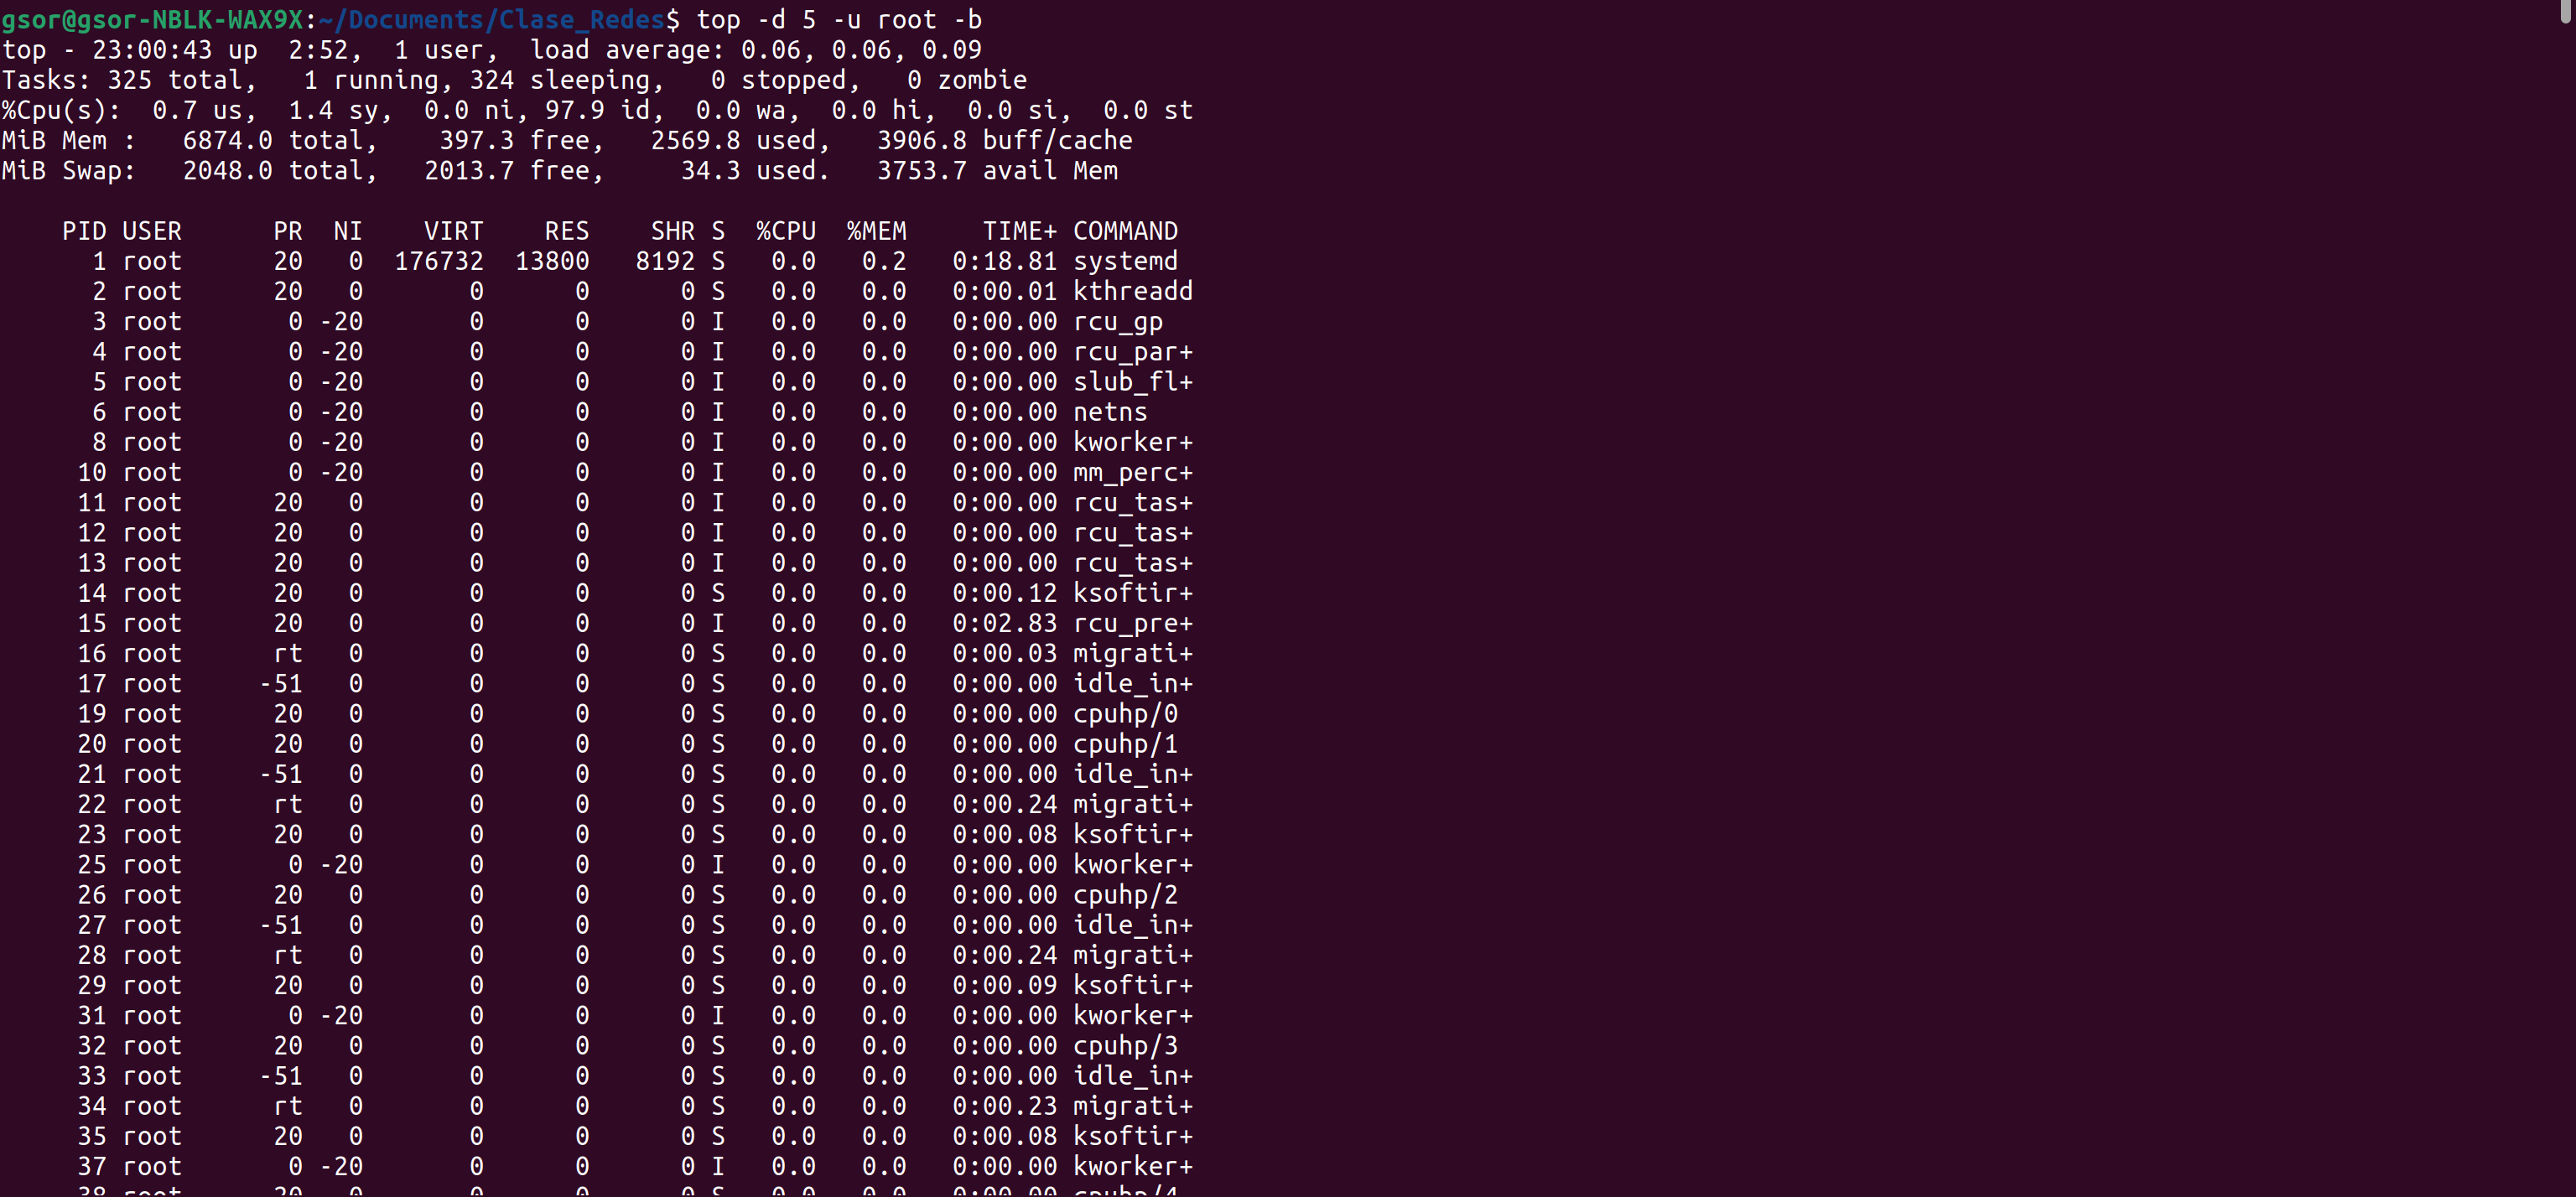
\includegraphics[width=10cm]{IMAGE/comandos/top.png}\\
    \end{center}
\end{itemize}
%-------------------------------------------

%% 
\newpage
\section*{Comandos en redes}

\begin{itemize}
    \item \textbf{Ifconfig}: Nos sirve para gestionar, verificar y visualizar las interfaces de red de nuestro sistema, por el momento solo visualizaremos.
    \begin{itemize}
        \item Investiga qué significan los resultados obtenidos y explícalos a grandes rasgos.
    \end{itemize}

    \begin{center}
        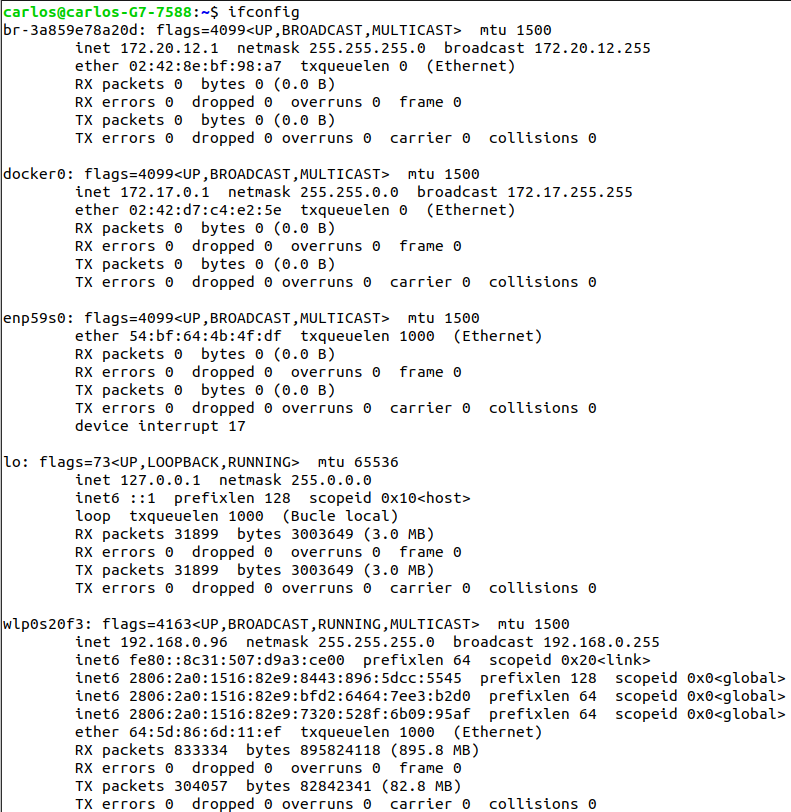
\includegraphics[width=12cm]{IMAGE/ifconfig.png}
    \end{center}
    
    \textbf{br-3a859e78a20d}: Esta es una interfaz de puente creada por Docker. Los puentes permiten a varios contenedores comunicarse en la misma red.
    
    \begin{itemize}
        \item \textbf{flags=4099$<$UP,BROADCAST,MULTICAST$>$}:  La interfaz está activa (UP) y admite difusión (BROADCAST) y multidifusión (MULTICAST).\\
        \item \textbf{mtu 1500}: La Unidad Máxima de Transmisión es de 1500 bytes.\\
        \item \textbf{inet 172.20.12.1}: La dirección IPv4 asignada es 172.20.12.1.\\
        \item \textbf{netmask 255.255.255.0}: La máscara de red es 255.255.255.0.\\
        \item \textbf{broadcast 172.20.12.255}: La dirección de difusión es 172.20.12.255.\\
        \item \textbf{ether 02:42:8e:bf:98}: La dirección MAC es 02:42:8e:bf:98\\
        \item \textbf{TX y RX packets}: Estadísticas de paquetes transmitidos (TX) y recibidos (RX). Actualmente, no ha habido tráfico en esta interfaz.
    \end{itemize}

    \textbf{docker0}: Otra interfaz de puente creada por Docker, utilizada para conectar contenedores Docker a la red.
    
    \begin{itemize}
        \item \textbf{flags=4099$<$UP,BROADCAST,MULTICAST$>$}:  Similar a la interfaz anterior.\\
        \item \textbf{mtu 1500}: La MTU es de 1500 bytes.\\
        \item \textbf{inet 172.17.0.1}: La dirección IPv4 es 172.17.0.1.\\
        \item \textbf{netmask 255.255.255.0}: La máscara de red es 255.255.0.0.\\
        \item \textbf{broadcast 172.20.12.255}: La dirección de difusión es 172.17.255.255.\\
        \item \textbf{ether 02:42:d7:c4:e2:5e}: La dirección MAC es 02:42:d7:c4:e2:5e.\\
        \item \textbf{TX y RX packets}:Estadísticas de tráfico, sin actividad en esta interfaz.
    \end{itemize}

    \textbf{enp59s0}: Interfaz Ethernet física en el sistema.
    
    \begin{itemize}
        \item \textbf{flags=4099$<$UP,BROADCAST,MULTICAST$>$}:  Similar a las interfaces anteriores.\\
        \item \textbf{mtu 1500}: La MTU es de 65536 bytes.\\
        \item \textbf{ether 54:bf:64:4b:4f}: La dirección MAC es 54:bf:64:4b:4f\\
        \item \textbf{TX y RX packets}: Estadísticas de tráfico, sin actividad en esta interfaz.
        \item \textbf{device interrupt 17}: La interrupción del dispositivo es 17, utilizada para manejar las señales del hardware.\\
    \end{itemize}

    \textbf{lo}: Esta es la interfaz de loopback, utilizada para la comunicación interna del sistema.
    
    \begin{itemize}
        \item \textbf{flags=73$<$UP,LOOPBACK,RUNNING$>$}:  Similar a la interfaz anterior.\\
        \item \textbf{mtu 1500}: La MTU es de 65536 bytes.\\
        \item \textbf{inet 127.0.0.1}: La dirección IPv4 de loopback es 127.0.0.1.\\
        \item \textbf{inet6 ::1}: La dirección IPv6 de loopback es ::1.\\
        \item \textbf{RX packets 4405, TX packets 4405}: Estadísticas de paquetes recibidos y transmitidos.\\
        \item \textbf{RX y TX errors}: Sin errores en la transmisión o recepción de paquetes.\\
    \end{itemize}

    \textbf{wlp0s20f3}: Esta es una interfaz inalámbrica en tu sistema.
    
    \begin{itemize}
        \item \textbf{flags=4163$<$UP,BROADCAST,RUNNING,MULTICAST$>$}:  La interfaz está activa, en ejecución, y admite difusión y multidifusión.\\
        \item \textbf{mtu 1500}: La MTU es de 1500 bytes.\\
        \item \textbf{inet 192.168.0.96}: La dirección IPv4 es 192.168.0.96.\\
        \item \textbf{netmask 255.255.255.0}: La máscara de red es 255.255.255.0.\\
        \item \textbf{broadcast 192.168.0.255}: La dirección de difusión es 192.168.0.255\\
        \item \textbf{inet6 fe80::8c31:507:d9a3}: Dirección IPv6 local (enlace local).\\
        \item \textbf{inet6 2806:2a0:1516:82e9:4b0d:1e8c:b841:56ed}: Dirección IPv6 global.\\
        \item \textbf{ether 64:5d:86:6d:11}: La dirección MAC es 64:5d:86:6d:11.\\
        \item \textbf{RX packets 78090, TX packets 41211}: Estadísticas de paquetes recibidos y transmitidos.\\
        \item \textbf{RX y TX errors}: Sin errores en la transmisión o recepción de paquetes.\\
    \end{itemize}
    
    \item \textbf{Ping}: Nos ayuda principalmente a verificar la conectividad entre nuestro sistema y algún otro conectado a una red (por ejemplo, tu computadora y la de tu amigo).
    \begin{itemize}
        \item Haz Ping a \texttt{www.google.com} y a la página de la facultad y mediante una captura muestra el resultado.
        \begin{center}
            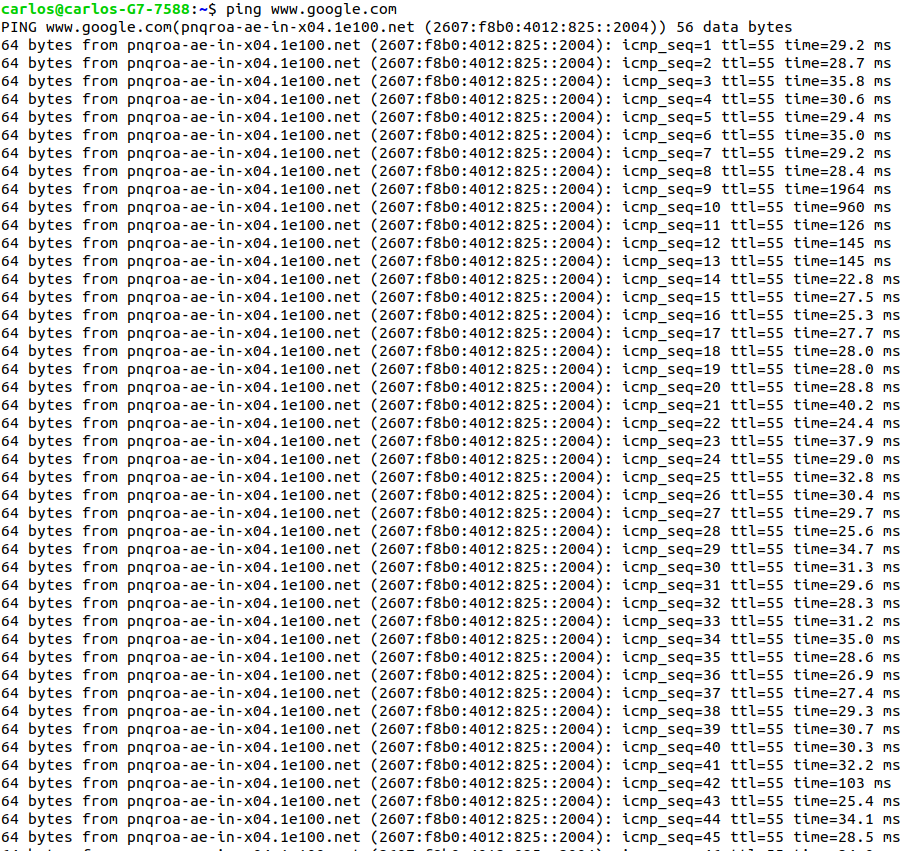
\includegraphics[width=12cm]{IMAGE/google.png}
        \begin{center}
            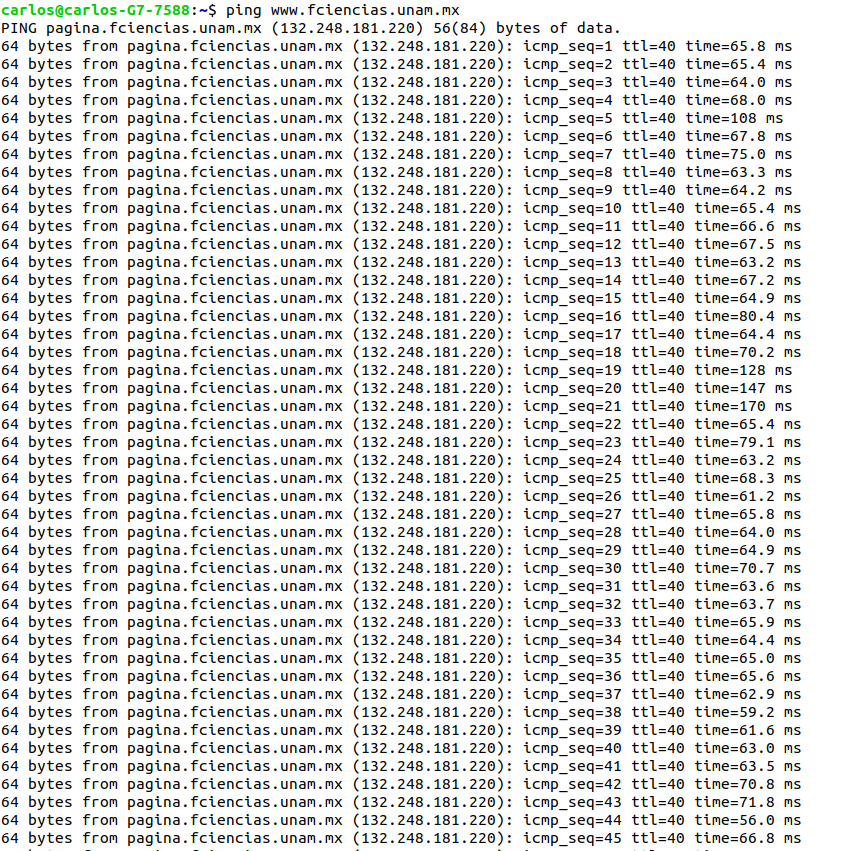
\includegraphics[width=12cm]{IMAGE/fciencias.png}
        \end{center}
    \end{center}
        \item ¿Ves algo diferente?\\

        \textbf{Dirección IP:} Notemos que google una una dirección numérica IPv4, mientras que la pagina de la facultad es una dirección hexadecimal IPv6

        \textbf{Tiempo de Respuesta:} Google presenta mayor variabilidad en sus tiempos de repuesta, dando fluctuaciones de frecuencia, y en la pagina de la facultad obervemos que los timpos de respuesta son mas consistentes sin haber una variación alta.

        También podemos decir que de estos tiempos de respuesta el más estable es el de la facultad, en cambio con los de google dado que los tiempos de respuesta son altos podemos tener problemas de red, o algún otro factor que este influyendo en la conectividad.
        
        \item Usa \texttt{ping -c <número> <ruta>}. ¿Para qué sirve el parámetro \texttt{-c}?\\

        El parámetro $-c$, en el comando ping enviará el número de paquetes que se especificaron y también nos da un resumen de las estadísticas de ping, como podemos observar en la imagen siguiente:
        
        \begin{center}
            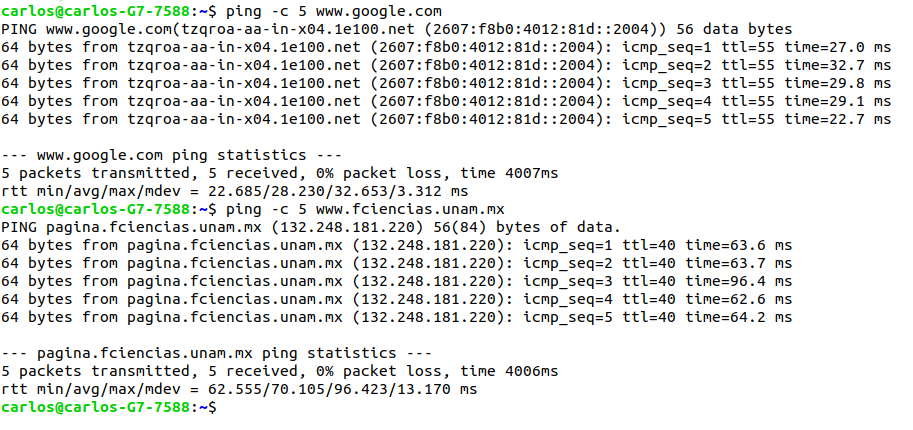
\includegraphics[width=12cm]{IMAGE/ping-c.png}
        \end{center}
        \item Extra: Haz Ping a la computadora de algún compañero de tu equipo y muestra el resultado.

        \begin{center}
            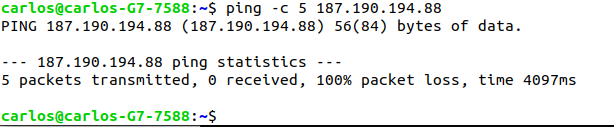
\includegraphics[width=12cm]{IMAGE/ping-computadora.png}
        \end{center}
    \end{itemize}

    \item \textbf{Traceroute}: Es un poco similar a Ping, pero lo que hace es rastrear la ruta que sigue un paquete de datos hasta un destino específico.

        El objetivo principal de esta herramienta es conocer el camino que recorre un paquete a través de nuestra red.
         Este comando de red nos permitirá saber por dónde pasa el paquete (máquinas, switches, routers) y 
         comprobar que nuestra red funciona correctamente. Si detecta cualquier problema, nos va a permitir tener 
         una idea aproximada acerca de dónde se encuentra el fallo. \cite{Pandora2024}

    \begin{itemize}
        \item Realiza las mismas actividades que Ping pero ahora con \texttt{traceroute}.
        
        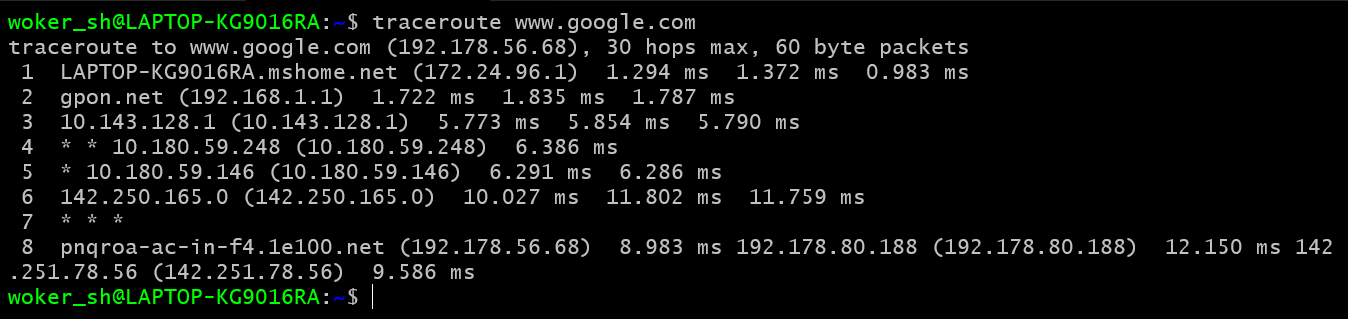
\includegraphics[scale = .3]{IMAGE/Ejercicio2/T01.png}

        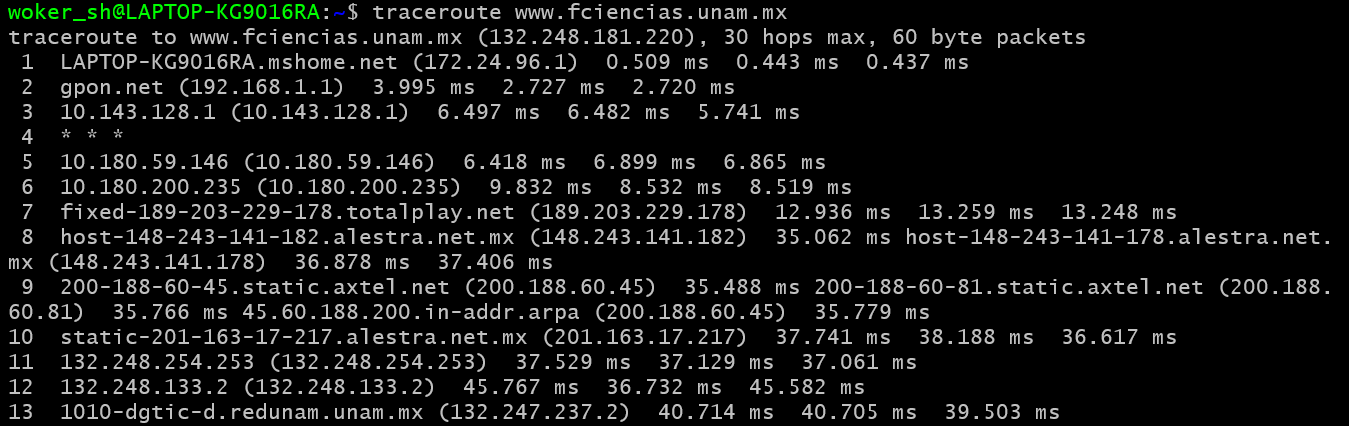
\includegraphics[scale = .3]{IMAGE/Ejercicio2/T02.png}
        
        \begin{itemize}
            \item ¿vez algo diferente?
            La pagiana de google muestra la ruta desde mi lap pasando por varirios enrutadores hasta uno 
            de los servidores de google mientras que la pagina de la facultad muestra una ruta con diferentes 
            rutas en el país finalizando en una que le pertenece a la UNAM. Para google algunos saltos no 
            estan señalados pero para la pagina de Ciencias si se muestran más múltiples redes locales.
        \end{itemize}


        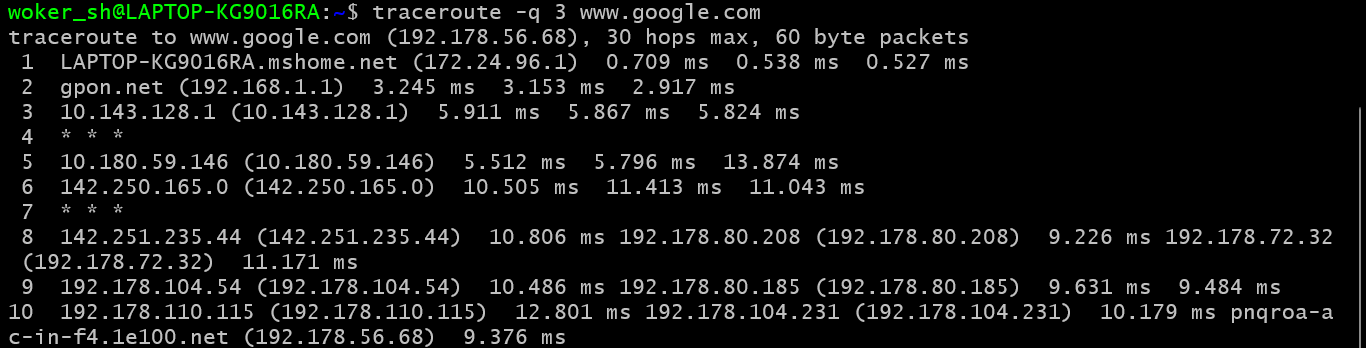
\includegraphics[scale = .3]{IMAGE/Ejercicio2/T03.png}
        \begin{itemize}
            \item \texttt{traceroute -q 3 www.google.com}
            
            El uso de \texttt{traceroute} con opción para múltiples paquetes a diferencia de \texttt{ping} se
            usa \texttt{-q} para especificar el número de consultas en cada salto, en la captura se 
            muestran los tiempos de respuesta para los 3 paquetes enviados a cada salto e indica si esque  
            no se recibieron respuestas en algunos saltos.
        \end{itemize}
    \end{itemize}

    \item \textbf{Netstat}: Este comando nos permite visualizar qué puertos están abiertos, lo cual 
    será muy útil si queremos verificar conexiones. Lista estándar de todas las conexiones activas \cite*{IONOS2022}

    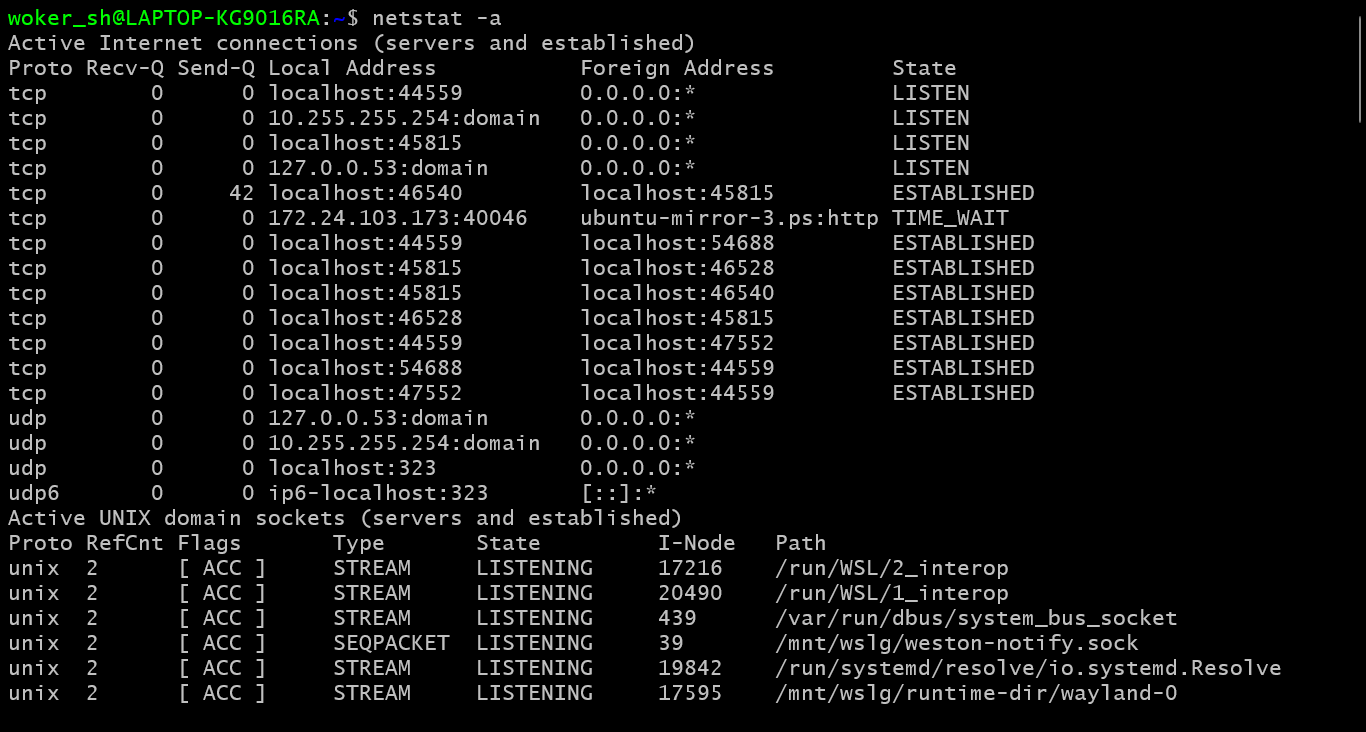
\includegraphics[scale = .3]{IMAGE/Ejercicio2/T04.png}

    \begin{itemize}        

        \item ¿Qué puedes observar?
        \item ¿Qué nos indica cada sección?
        
        \begin{itemize}
            \item Proto: Indica el protocolo de red utilizado (TCP o UDP).
            \item Recv-Q: Muestra la cantidad de datos que han llegado a la cola de recepción pero aún no se han leído por el proceso.
            \item Send-Q: Muestra la cantidad de datos que están en la cola de envío, esperando ser enviados.
            \item Local Address: La dirección IP local y el puerto en el que el proceso está escuchando o conectado.
            \item Foreign Address: La dirección IP y el puerto remoto con el que el proceso está conectado.
            \item State: El estado de la conexión (solo para TCP).
        \end{itemize}

        \begin{itemize}
            \item TCP LISTEN: Puertos que están esperando nuevas conexiones.
            \item TCP ESTABLISHED: Conexiones activas entre el puerto local y un puerto remoto.
            \item TCP TIME WAIT: La conexión ha sido cerrada, pero está en espera de que todos los datos se transmitan correctamente.
            \item UDP: Puertos en los que los servicios están listos para recibir datagramas.
            \item UDP6: Puertos en IPv6 esperando datagramas.
        \end{itemize}

    \end{itemize}

    \item Investiga 3 comandos más que consideres que se usan en redes (no importa si requieren instalación adicional como \texttt{speedtest}) y menciona qué hace cada uno.
    
    \begin{itemize}
        \item comando \texttt{dig} \cite*{ComandDIG}
        
        En su forma más simple, la sintaxis del comando Dig se verá así:
        \begin{center}
            \texttt{dig [servidor] [nombre] [tipo]}
        \end{center}
        
        \begin{itemize}
            \item[] servidor: la dirección IP o el hostname del nombre del servidor a consultar.
            
            Si el argumento del servidor es el hostname, dig resuelve el hostname antes de continuar con la consulta.            

            \item[] nombre: el nombre del registro de recursos que se debe buscar.
            \item[] tipo: el tipo de consulta solicitada por dig. Por ejemplo, puede ser un registro A, 
            un registro MX, un registro SOA o cualquier otro tipo. De forma predeterminada, \texttt{dig} realiza 
            una búsqueda de un registro A si no se especifica ningún argumento de tipo.
        \end{itemize}

        \item comando \texttt{arp} \cite*{IONOSARP}
        
        El Address Resolution Protocol es un protocolo estándar que se puede utilizar en cualquier plataforma y que, 
        como tal, se ocupa de la asignación de direcciones MAC en un segundo plano independientemente del sistema, 
        ya sea Linux, Windows o macOS.\\

        El comando \texttt{arp –a} funciona en cualquier sistema. Al introducirlo aparece una lista de combinaciones
        de direcciones para todas las interfaces de red que utilizan ARP. ¿Cómo funciona? A la hora de 
        asignar direcciones por medio del Address Resolution Protocol hay que distinguir si la dirección IP 
        del host de destino se encuentra en la misma red local o en otra subred. Así, en caso de asignar una 
        dirección MAC a una determinada dirección IP, antes de nada se lleva a cabo una revisión de la 
        máscara de subred. Si la IP se encuentra en la red local, el primer paso es controlar si ya existe 
        una entrada para ella en la caché del ARP.


        \item comando \texttt{ncat} \cite*{IONOSNAT}
        
        Netcat es una herramienta de línea de comandos que sirve para escribir y leer datos en la red. Para 
        la transmisión de datos, Netcat usa los protocolos de red TCP/IP y UDP. La herramienta proviene 
        originalmente del mundo de Unix.

        La sintaxis de Netcat consiste en dos componentes fundamentales: el comando básico “nc”, siempre idéntico, seguido por varias “opciones”. El comando básico direcciona al archivo de programa nc.exe, mientras que las opciones determinan el rango concreto de funciones de la versión de Netcat, por lo que varían dependiendo del sistema operativo y de la versión de Netcat utilizada.

        \begin{table}[h!]
            \centering
            \begin{tabular}{|l|l|}
            \hline
            \textbf{Opciones} & \textbf{Descripción} \\ \hline
            -4 & Fuerza el uso de IPv4 (GNU Netcat) \\ \hline
            -6 & Fuerza el uso de IPv6 (GNU Netcat) \\ \hline
            -d & Elimina Netcat de la consola  \\ \hline
            -D & Habilita la opción de depurar los sockets (GNU Netcat) \\ \hline
            -h (display help) & Muestra la ayuda  \\ \hline
            \end{tabular}
            \caption{Opciones de GNU Netcat}
            \label{tab:netcat_options}
            \end{table}            
    \end{itemize}
\end{itemize}   

%-------------------------------------------

%% 
\newpage
\section*{Teoría}

\begin{enumerate}
    \item ¿Para qué es y en qué casos se usa el usuario \texttt{root}? ¿En qué casos no se usa o no debe usarse?
    
    Para Linux y macOS, el usuario root es el superusuario. Esto significa que tiene el mayor nivel de privilegios para 
    realizar cualquier acción en el sistema, modificar cualquier archivo, instalar software, cambiar la configuración 
    del sistema y ejecutar cualquier comando, sin restricciones.

    Si bien suena increible tener todo el control en el sistema hay desventajas, por ejemplo entornos compartidos, 
    para servidores o sistemas compartidos, es recomendable limitar el uso del usuario root a tareas estrictamente 
    necesarias y utilizar cuentas con privilegios más restringidos para las tareas diarias. \cite*{UserRoot}

    
    \item ¿Cuál es la diferencia entre \texttt{su} y \texttt{sudo}? \cite*{RootSU}
    
    \begin{itemize}
        \item \texttt{su}: Al ejecutar \texttt{su}, se cambia de usuario y convertirte en 
        el superusuario (root), que tiene permiso para hacer cualquier cosa en el sistema.

        \item \texttt{sudo}: Lo mismo que arriba pero es temporal, permite ejecutar el comando como 
        super usuario y recordará la contraseña como por 15 min, despues la volverá a pedir.
    \end{itemize}
    
    \item ¿Para qué sirve \texttt{chmod}? ¿Cómo se usa?
    
    El programa de línea de comandos chmod, abreviatura de change mode (cambiar modo en inglés), 
    chmod sirve para asignar permisos de acceso a carpetas y directorios en sistemas de archivos 
    compatibles con los permisos de archivo típicos de Unix.\\

    En Unix, el sistema de permisos de acceso a los archivos se basa en dos elementos fundamentales: 
    las clases de usuario y los permisos básicos individuales. En la gestión de estos permisos, 
    chmod soporta dos modos diferentes: la notación simbólica con letras (modo simbólico o carácter) 
    y la atribución de permisos con códigos octales de cifras (modo octal).


    ¿Cómo se usa? \texttt{chmod [opciones] modo archivo}


    \begin{itemize}
        \item opciones: Son parámetros adicionales que modifican el comportamiento del comando.
        \item modo: Especifica los nuevos permisos. Puede ser en formato numérico u octal (más común) o simbólico.
        \item archivo: El archivo o directorio al que se aplicarán los cambios.
    \end{itemize}
    
    Por ejemplo:
    \begin{center}
        chmod 755 archivo.txt    
    \end{center}

    Asigna permisos de lectura, escritura y ejecución al propietario, lectura y ejecución al grupo, y 
    lectura y ejecución a otros.


    \item Genera un pequeño pipeline de los comandos vistos durante la práctica, por ejemplo:
    \begin{enumerate}
        \item Crear una carpeta con un nombre.
        \item Crear un archivo.
        \item Con \texttt{traceroute}, generar una búsqueda y guardar el resultado en dicho archivo.
        \item Visualizar el contenido con \texttt{cat}, \texttt{head}, o \texttt{less} de dicho archivo.
        \item Modificar los permisos de lectura y escritura de este.
    \end{enumerate}
    
\begin{verbatim}
    # 1. Crear una carpeta 
    mkdir practica01
    
    # 2. Crear un archivo dentro de la carpeta
    touch practica01/ejercicoTeoria.txt
    
    # 3. Con traceroute, generar una búsqueda y guardar el resultado en dicho archivo
    traceroute www.google.com > practica01/ejercicoTeoria.txt
    
    # 4. Visualizar el contenido con cat
    cat practica01/ejercicoTeoria.txt    
    
    # 5. Modificar los permisos de lectura y escritura
    chmod 644 practica01/ejercicoTeoria.txt

    # 6. Ver los permisos 
    ls -l practica01/ejercicoTeoria.txt
\end{verbatim}

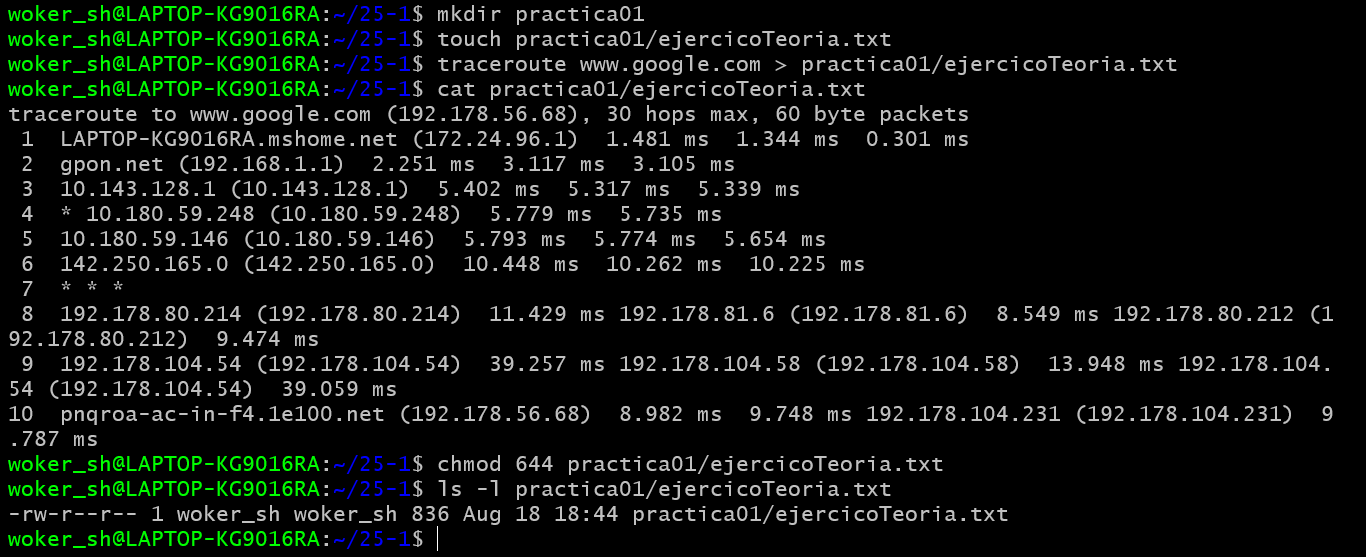
\includegraphics[scale = .3]{IMAGE/Ejercicio2/T05.png}

    \item Por último, añade lo aprendido de esta práctica, así como las posibles complicaciones que tuviste al realizarla.
\end{enumerate}
\begin{center}

    \item Carlos Daniel Cortés Jiménez: Me pareción intereante la practica ya que hubo muchos comandos que no conocía, y a su vez se me complicó al principio ejecutarlos ya que no escribía como debe de usarse algunos comandos. Después de ver guías y leer en internet me resultó más fácíl de lo que pense, también he de decir que lo que mas se me dificultó entender y aún tengo dudas son todos los apartados que da como resultado el realizar ifconfig.
    
    \item Marco Silva Huerta: A pesar de ya tener conocimientos previos de semestres anteriores sobre algunos comandos vistos en la practica, me resultó muy interesante. Pude refrescar y recordar el uso de comandos conocidos y a su vez aprender nuevas opciones y banderas me que a mi parecer resultó útil ver como combinar varias banderas para optimizar el uso de comandos, algo que no solía hacer con frecuencia. En general, fue una practica muy divertida que me facilitó recordar y aplicar comandos de manera más eficiente.
    
    \item Giovanny Cruz: Aprendi el uso de muchos comandos que no conocia. Al principio me costo un poco entender el uso de las banderas,
            pero despues de un rato de practica, se me hizo mas facil. Cre que lo que mas me costo, fue un poco el entender como usar varias 
            banderas al mismo tiempo, pero es muy util para hacer mas eficiente el uso de los comandos.

    \item Jonathan Martínez: La mayoría de los comandos que tuvimos que investigar no los conocía, quizá algunos los había usado con 
            anterioridad pero no consciente de su funcionamiento total. Revisar el manual de los comandos ayudó mucho a comprender su 
            funcionamiento.

    \item Edgar Montiel Ledesma: Volvo a recordar muchas vanderas utilies en esta practica ya que si los conocia pero, no es frecuente el uso de estos en el dia a dia, es bueno tener esta tarea para tenerlos presentes y hacer mas facil las actividades, por otro lado gracias al comando de man es mas facil poder recordarlos en el momente que se necesiten.
    
\end{center}

%-------------------------------------------

% ----------------------|
% Referencias           |
% Forma de Compilar     |
% pdflatex main.tex     |
% biber main            |
% pdflatex main.tex     |
\newpage %              |
\thispagestyle{fancyref}
\printbibliography %    |
% ----------------------|

\end{document}%----------------------F I N DOCUMENTO---------------|
%------------------------------------------------------------------|